%\documentclass[twocolumn,prc,showpacs,nofootinbib,preprintnumbers,amsmath,amssymb,superscriptaddress]{revtex4-1}
\documentclass[12pt,preprint,tightenlines,
showpacs,preprintnumbers,amsmath,amssymb,
%superscriptaddress,
a4paper,nofootinbib]{revtex4-1}

\bibliographystyle{model1a-num-names}


\usepackage{nicefrac}
%\usepackage[scaled]{helvet}
%\usepackage{courier}


\usepackage{fouriernc}
%\renewcommand{\familydefault}{\sfdefault}
%\usepackage[no-math]{fontspec}


\usepackage{natbib}
\usepackage{amssymb,amsbsy,amsmath,amsfonts}
\usepackage{graphicx}% Include figure files
\usepackage{epsf,epsfig,float,latexsym,amsthm,fancyhdr,rotating}
\usepackage{graphics,psfrag,longtable}
%\usepackage{srcltx}
\usepackage{slashed}
%\usepackage{footnote}
\usepackage[colorlinks,citecolor=blue,linktoc=all,linkcolor=cyan,urlcolor=blue]{hyperref}
\usepackage{upgreek}
 
 
 \usepackage{setspace}
 
 \renewcommand{\baselinestretch}{1.15}
 
\def\hpm{\hphantom{-}}
\def\beq{\begin{equation}}
\def\eeq{\end{equation}}
\def\bea{\begin{eqnarray}}
\def\eea{\end{eqnarray}}
\def\beqa{\begin{equation}\begin{array}{l}}
\def\eeqa{\end{array}\end{equation}}
% labels
\def\eqlab#1{\label{eq:#1}}
\def\figlab#1{\label{fig:#1}}
\def\tablab#1{\label{tab:#1}}
\def\seclab#1{\label{sec:#1}}
% reference
\def\eref#1{(\ref{eq:#1})}
\def\Eqref#1{Eq.~(\ref{eq:#1})}
\def\figref#1{fig.~\ref{fig:#1}}
\def\fref#1{\ref{fig:#1}}
\def\Figref#1{Fig.~\ref{fig:#1}}
\def\tabref#1{\ref{tab:#1}}
\def\Tabref#1{Table \ref{tab:#1}}
\def\secref#1{Section \ref{sec:#1}}
% vectors
\def\sla#1{#1 \hspace{-2mm} \slash}
\def\slap{p \hspace{-2mm} \slash}
\def\slad{\partial \hspace{-2.2mm} \slash}
\def\slaP{P \!\!\!\! \slash}
% fractions
\def\boxfrac#1#2{\mbox{\small{$\frac{#1}{#2}$}}}
\def\half{\mbox{$\frac{1}{2}$}}
\def\sfrac#1{\mbox{\small{$\frac{1}{#1}$}}}
\def\thalf{\mbox{\small{$\frac{3}{2}$}}}
\def\quarter{\mbox{$\frac{1}{4}$}}
\def\third{\mbox{$\frac{1}{3}$}}
\def\sixth{\mbox{$\frac{1}{6}$}}

% matrices
\def\barr{\left(\begin{array}{c}}
\def\earr{\end{array}\right)}
\def\bmat{\left(\begin{array}{cc}}
\def\emat{\end{array}\right)}
%--------------------------------------------
% symbols
\def\al{\alpha}
\def\be{\beta}
\def\ga{\gamma} \def\Ga{{\it\Gamma}}
\def\de{\delta} \def\De{\Delta}
\def\veps{\varepsilon}  \def\eps{\epsilon}
\def\kp{\kappa}
\def\la{\lambda} \def\La{{\Lambda}}
\def\Pit{{\it\Pi}}
\def\Psit{{\it\Psi}}
\def\si{\sigma} \def\Si{{\it\Sigma}}
\def\th{\theta} \def\vth{\vartheta} \def\Th{\Theta}
\def\w{\omega} \def\W{\Omega} \def\hw{\hat{\omega}}
\def\vfi{\varphi}\def\vphi{\varphi}
\def\z{\zeta}
\def\bra{\langle} \def\ket{\rangle}

\def\pa{\partial}
\def\vrho{\varrho}
\def\barf{\zeta}
\def\ie{{i.e., }}
\def\eg{{e.g.\ }}
\def\cl{\centerline}
\def\ni{\noindent}
\def\pa{\partial}
\def\ra{\rightarrow}
\def\nn{\nonumber}
\def\dd{\mathrm{d}}
\def\cO{\mathcal{O}}
\def\DD{{\mathcal D}}
\def\lag{{\mathcal L}}
\def\ham{{\mathcal H}}
\def\aa{\mathcal{a}}
\def\kk{\mathcal{k}}
%\def\gg{\mathcal{g}}
\def\xx{\mathscr{x}}
\def\yy{\mathscr{y}}
\def\zz{\mathscr{z}}
\def\MM{\mathcal{M}}
\def\MA{{\mathcal A}}
\def\MR{{\mathcal R}}
\def\MQ{{\mathscr q}}
\def\MB{{\mathcal B}}
\def\MP{{\mathcal P}}
\def\TT{{\mathscr T}}
\def\ZZ{\mathcal{Z}}
\def\rZ{\mathantt{Z}}
\def\zZ{\mathpzc{Z}}



\def\bGa{{\bf\Gamma}}
\def\bS{{\bf S}}
\def\psib{\bar{\psi}} \def\Psib{\bar{\Psit}}
\def\pib{\bar{\pi}} \def\Pib{\bar{\Pi}}
\def\xib{\bar{\xi}}

\DeclareMathOperator\arctanh{arctanh}
\DeclareMathOperator\im{Im}
\DeclareMathOperator\re{Re}\def\3d{3-D}
\def\CMS{CMS}
\def\ODI{O$\Delta$I}
\def\ODR{O$\Delta$R}
\newcommand{\lsim}{\, \, \raisebox{-0.8ex}{$\stackrel{\textstyle <}{\sim}$ }}
\def\ol#1{\overline{#1}}
\def\amm{a.m.m.}
%---------------------------------
\def\hate{\hat{\mathbf{e}}}
\def\bq{\mathbf{q}}
\def\bvare{\boldsymbol{\varepsilon}}
\def\bsig{\boldsymbol{\sigma}}


%\textwidth18.5cm
\begin{document}
%\preprint{MITP/13-042}
\title {Forward doubly-virtual 
Compton scattering off the nucleon in chiral perturbation theory at NLO:
the subtraction function and moments of unpolarized structure functions}
\author{Jose Manuel Alarc\'on}
%\affiliation{
%Cluster of Excellence PRISMA Institut f\"ur Kernphysik, Johannes Gutenberg-Universit\"at, Mainz D-55099, Germany}
\affiliation{Departamento de F\'isica Te\'orica \& IPARCOS, Universidad Complutense de Madrid, 28040
Madrid, Spain}
\author{Franziska Hagelstein}
\affiliation{Albert Einstein Center for Fundamental Physics, Institute for Theoretical Physics, University of Bern, Sidlerstrasse 5, CH-3012 Bern, Switzerland}
\author{Vadim Lensky}
\affiliation{Institut f\"ur Kernphysik \&  Cluster of Excellence PRISMA,
 Johannes Gutenberg-Universit\"at  Mainz,  D-55128 Mainz, Germany}
%\affiliation{Institute for Theoretical and Experimental Physics, Bol'shaya Cheremushkinskaya 25, 117218 Moscow, Russia}
%\affiliation{National Research Nuclear University MEPhI (Moscow Engineering Physics Institute), 115409 Moscow, Russia}
\author{Vladimir Pascalutsa}
\affiliation{Institut f\"ur Kernphysik \&  Cluster of Excellence PRISMA,
 Johannes Gutenberg-Universit\"at  Mainz,  D-55128 Mainz, Germany}
 \email{vladipas@kph.uni-mainz.de}
\begin{abstract}
The forward doubly-virtual 
Compton scattering (VVCS) off the nucleon contains a wealth of information on nucleon structure, relevant to the calculation
of the two-photon-exchange effects in atomic spectroscopy and electron scattering. We report on a complete next-to-leading order (NLO)
calculation of low-energy VVCS in chiral perturbation
theory ($\chi$PT). 
Here we focus on the unpolarized VVCS amplitudes $T_1(\nu, Q^2)$
and $T_2(\nu, Q^2)$, and the corresponding structure functions
$F_1(x, Q^2)$ and $F_2(x,Q^2)$. Our results are confronted, where possible, with ``data-driven'' dispersive evaluations of 
low-energy structure 
quantities, such as nucleon polarizabilities.  We find  significant disagreements with dispersive evaluations at very
low momentum-transfer $Q$; for example,
in the slope of polarizabilities at zero momentum-transfer. 
By expanding the results in powers of the inverse nucleon  mass, we reproduce the known ``heavy-baryon'' expressions. This serves as a check of our calculation, as well as a demonstration of large differences between the manifestly Lorentz-invariant (B$\chi$PT)
and heavy-baryon (HB$\chi$PT) frameworks. 
 
 

\end{abstract}
\pacs{}
\date{\today}
\maketitle

\tableofcontents

\newpage
\section{Introduction and outline}


The forward doubly-virtual 
Compton scattering (VVCS), \Figref{CSgeneric}, is not a directly observable process. Nevertheless, it 
is traditionally of high relevance in studies
of nucleon and nuclear structure, and of their impact on atomic nuclei. Ah high energies
the VVCS has the  apparent connections to deep-inelastic scattering, whereas 
at low energy it is important for precision atomic spectroscopy, where it serves as input for calculations of the nuclear-structure corrections. Analytical properties of the VVCS amplitude
are used to establish useful relations --- sum rules ---
between the static 
(electromagnetic moments, polarizabilites) 
and dynamic (photoabsorption cross sections) properties of the nucleon \cite{GellMann:1954db,Burkhardt:1970ti,Schwinger:1975uq,Bernabeu:1974mb,Lvov:1998vg},
see also \cite{Drechsel:2002ar,Kuhn:2008sy,Holstein:2013kia,Hagelstein:2015egb,Pascalutsa:2018ced,Pasquini:2018wbl} for reviews. 

\begin{figure}[bht]
\centering
       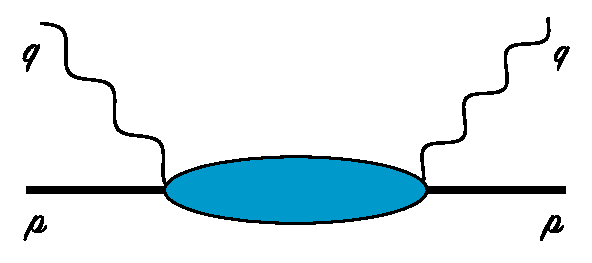
\includegraphics[width=5.5cm]{frwCSgeneric.eps}
\caption{The forward Compton scattering, or VVCS, in case of virtual photons, $q^2=-Q^2$.
  \label{fig:CSgeneric}}
\end{figure}

In the last decade, with the advent of muonic-atom spectroscopy
by the CREMA Collaboration \cite{Pohl:2010zza,Antognini:1900ns,Pohl1:2016xoo},
the interest in nucleon VVCS has resurged in the context of 
the  ``proton radius puzzle'' (see, e.g.,  \cite{Pohl:2013yb,Carlson:2015jba} for reviews).  
The muonic atoms, being more sensitive to nuclear structure than
conventional atoms, demand a higher quality of this input
in both the Lamb shift \cite{Pohl:2010zza,Antognini:1900ns} and, in the near future, the hyperfine-structure measurements  \cite{Pohl:2016xsr,Bakalov:2015xya,Kanda:2018oay}. The VVCS  enters here in the form of the two-photon exchange (TPE) corrections appearing at $O(Z^4\al^5)$, which is the subleading order for the nuclear-structure effects in the Lamb shift (the leading  being the  charge radius), and leading in the hyperfine structure. In either case, the TPE is the leading theoretical uncertainly and precising this contribution is a challenge for the nuclear and hadron
physics community.

In this work we focus on the unpolarized nucleon 
VVCS, described, for each nucleon (proton or neutron), by two scalar amplitudes $T_{1,2}(\nu,Q^2)$,
functions of the photon energy $\nu$ and virtuality $Q^2$.
The  discontinuity of these amplitudes is
given, respectively, by the two unpolarized structure functions $F_1(x,Q^2)$ and
$F_{2}(x, Q^2)$.

To date, there are two approaches: 
\textit{1) dispersion relations (DR)} and 
\textit{2) chiral perturbation theory ($
\chi$PT)}, used for evaluation
of nucleon VVCS, with the goal of quantifying the relevant corrections in muonuc hydrogen.
It is expected and  highly desirable that 
\textit{3) lattice QCD} will join this effort in the near future. 
In the mean time, however, the DR approach is the most popular one.
It employs the well-known dispersion relations expressing 
the VVCS amplitudes as integrals of the structure
functions known empirically from inclusive electron scattering. 


Unfortunately, the DRs determine the VVCS in terms of the structure functions only up to a ``subtraction  function'' $T_1(0,Q^2)$. 
The latter function is not well-constrained empirically, which
makes this approach prone to model uncertainties. It is work to mention that there is a
new proposal on how the subtraction can further be constrained
via the dilepton electroproduction \cite{Pauk:2020gjv}. However in the foreseeable future,
this issue will preclude a systematic improvement of the theoretical uncertainty within the DR approach. 


Here we employ the second approach. More specifically, we use an extension of SU(2) Chiral Perturbation Theory ($\chi$PT) \cite{Weinberg:1978kz,Gasser:1983yg} to the single-baryon sector \cite{Gasser:1987rb,Gegelia:1999gf,Fuchs:2003qc}, referred to as the baryon $\chi$PT (B$\chi$PT), augmented by inclusion 
of the explicit $\Delta(1232)$-isobar in the $\de$-counting scheme
\cite{Pascalutsa:2003aa}. 
In this framework we compute the inelastic (non-Born) part of
VVCS amplitudes to next-to-leading order (NLO).
A first version of this calculation was briefly considered in~Ref.~\cite{Lensky:2014dda}. Here we provide a few important improvements, in particular, the inclusion the Coulomb-quadrupole $(C2)$ $N\to \Delta$ transition, and a more comprehensive comparison of our results with the DR approach. 
The impact of this
calculation on the muonic-hydrogen Lamb shift, extending
our previous evaluation~\cite{Alarcon:2013cba} to higher orders, will be discussed elsewhere.

The paper is organized as follows. In Sec.~\ref{Sec:ChEFT_for_VVCS}, we recall the general formulae and
the main ingredients of our NNLO calculation. In Sec.~\ref{App:CrossSections}, we the structure functions, in particular, the $\pi N$, $\pi \De$ and $\De$ production channels  
relevant to our calculation.
In Sec.~\ref{Sec:Scalar-Pol}, we examine results for the proton and neutron scalar polarizabilities, and some of the other moments
of structure functions.  In the concluding section 
(Sec.\ \ref{Sec:Summary}), we summarize and give an brief outlook
for the near-future work. 










%In the appendices, we analyze some technical details involved in the calculations (Appendix~\ref{sec:SRVVCStensor}) and show the contributions of the $\pi N$ loops and the $\Delta$ exchange to the polarizabilities and their slopes at the real-photon point (Appendix~\ref{App:PolarizabilitiesAll}). 







\section{Relation to structure functions, form factors  and polarizabilities} \seclab{LorentzDecomp}

Figure \ref{fig:CSgeneric} shows schematically the VVCS 
amplitude, which for an unpolarized target  (of any spin) can be decomposed into two
independent Lorentz-covariant and gauge-invariant tensor structures
\cite{Hagelstein:2015egb}:
%\begin{align}\label{Eq:T-Rel}
%T(\nu,Q^2) = \epsilon_{\mu}^{\prime *} \epsilon_\nu \Bigg\{  \Big( -g^{\mu \nu} + \frac{q^\mu q^\nu}{q^2} \Big) T_1(\nu,Q^2) + \frac{1}{M_N^2} \Big(  p^\mu - \frac{p\cdot q}{q^2} q^\mu \Big) \Big(  p^\nu - \frac{p\cdot q}{q^2} q^\nu \Big) T_2(\nu,Q^2) \nonumber \\ 
%                  +  \frac{i}{M_N} \epsilon^{\mu \nu \alpha \beta} q_\alpha s_\beta S_1(\nu,Q^2)   +\frac{i}{M_N^3} \epsilon^{\mu \nu \alpha \beta} q_\alpha (p\cdot q  s_\beta -s\cdot q  p_\beta ) S_2(\nu,Q^2)      \Bigg\}, 
%\end{align}
%where $s^\mu$ is the covariant spin tensor which satisfy $s\cdot p=0$ and $s^2=-1$, and the normalization of the Levi-Civita tensor is $\epsilon_{0123}=+1$. 
\bea
\label{Eq:T-Rel}
T^{\mu\nu}(p,q) & = &  
\left( -g^{\mu\nu}+\frac{q^{\mu}q^{\nu}}{q^2}\right)
T_1(\nu, Q^2) +\frac{1}{M_N^2} \left(p^{\mu}-\frac{p\cdot
q}{q^2}\,q^{\mu}\right) \left(p^{\nu}-\frac{p\cdot
q}{q^2}\, q^{\nu} \right) T_2(\nu, Q^2),
\eqlab{fVVCS}
\eea
where $p$ and $q$ are the four-momenta of the target particle (here, nucleon)  and the photon, respectively; $M_N$ is the nucleon mass. 
The scalar amplitudes $T_i$ are functions of the photon
energy $\nu = p\cdot q/ M_N$ and virtuality $Q^2=-q^2$.


The optical theorem relates the absorptive parts of the VVCS amplitudes to the structure functions, or equivalently, the inclusive electroproduction cross sections:
\begin{subequations}
\eqlab{VVCSunitarity}
\bea
\im T_1(\nu,Q^2)&=&\frac{4\pi^2\al}{M_N}F_1(x,Q^2) \nn\\ \eqlab{ImT1} &=& K(\nu,Q^2)\,\sigma_T(\nu,Q^2), \\
\im T_2(\nu,Q^2)&=&\frac{4\pi^2\al}{\nu}F_2(x,Q^2)\nn\\
\eqlab{ImT2} &=& \frac{Q^2  K(\nu,Q^2) }{\nu^2+Q^2}\left[\sigma_T(\nu,Q^2)+\sigma_L(\nu,Q^2)\right],
\eea
\end{subequations}
with the fine-structure constant $\alpha=e^2/4\pi$, and the Bjorken variable $x=Q^2/(2M_N \nu)$. The two response functions $\sigma_T$ and $\sigma_L$ are cross sections of total photoabsorption  of a transversely (T) and longitudinally (L) polarized photons.
The flux of virtual photons is
conventionally defined up to the flux factor $K(\nu,Q^2)$. The experimental observables do not depend on it, only the definitions of the response functions $\sigma_T$ and $\sigma_L$ do.  
Throughout this work we adopt  Gilman's flux factor 
(for other common choices, cf.~\cite{Drechsel:2002ar}):
\beq 
K(\nu,Q^2)=\vert\vec{q}\,\vert=\sqrt{\nu^2+Q^2},
\eeq
where  $\vec{q}$ is the photon three-momentum in the lab frame.

The VVCS amplitudes satisfy the following dispersion relations derived from the above statement of the  optical theorem, combined with general principles of analyticity and crossing symmetry
(cf., for example, \cite{Drechsel:2002ar,Hagelstein:2015egb,Pascalutsa:2018ced} for  details):
\begin{subequations}
\eqlab{genDRs}
\bea 
T_1 ( \nu, Q^2) &=&T_1(0,Q^2) + \frac{32\pi\al M_N\nu^2}{Q^4} \int_{0}^1 
\!\dd x \,
\frac{x\, F_1 (x, Q^2)}{1 - x^2 (\nu/\nu_{\mathrm{el}})^2 - i 0^+} \nonumber\\ 
&=& T_1(0,Q^2) + \frac{2\nu^2}{\pi } \int_{\nu_{\mathrm{el}}}^\infty\! \frac{\dd \nu'}{\nu'} \, 
\frac{\sqrt{\nu^{\prime\,2}+Q^2}\,\si_T ( \nu', Q^2)}{\nu^{\prime\,2} -\nu^2 - i 0^+}\,,\eqlab{T1dr}\\
T_2 ( \nu, Q^2) &=& \frac{16\pi\al M_N}{Q^2} \int_{0}^1 
\!\dd x\, 
\frac{F_2 (x, Q^2)}{1 - x^2 (\nu/\nu_{\mathrm{el}})^2  - i 0^+} \nonumber \\
&=&\frac{2Q^2}{\pi} \int_{\nu_{\mathrm{el}}}^\infty\! \dd \nu' \, 
\frac{\nu^{\prime}\,[ \si_T+\si_L] ( \nu', Q^2)}{\sqrt{\nu^{\prime\,2}+Q^2}(\nu^{\prime\,2} -\nu^2- i 0^+)} \eqlab{T2dr},
\eea 
\end{subequations}
with $\nu_{\mathrm{el}}=Q^2/2M_N$ the elastic threshold. The high-energy behavior of $F_1(x,Q^2)$ prevents the convergence of the corresponding unsubtracted dispersion integral,  hence
leading to the once-subtracted dispersion relation, \Eqref{T1dr}, with the aforementioned ``subtraction function'' $T_1(0,Q^2)$. 
Note that while the subtraction point is conventionally
chosen at $\nu = 0$, 
other choices are in principle possible. Future lattice QCD calculations of the VVCS amplitude would likely  prefer to deal
with an Euclidean subtraction point,  e.g., at $\nu =iQ/2$, as chosen in \cite{Gasser:2020mzy}. 


The amplitudes are naturally split into nucleon-pole ($T_i^{\mathrm{pole}}$) and non-pole ($T_i^{\mathrm{nonpole}}$)
parts, or Born ($T_i^{\mathrm{Born}}$) and non-Born ($\ol T_i$) terms,
\beq
T_i = T_i^{\mathrm{pole}} + T_i^{\mathrm{nonpole}}
= T_i^{\mathrm{Born}} + \ol T_i
\eeq 
with the pole and Born terms given uniquely in terms
of the nucleon electric ($G_E$) and magnetic ($G_M$) form factors:
\begin{subequations}
\bea
T_1^{\mathrm{pole}}   (\nu,Q^2) &=& \frac{4\pi \al}{M_N}
\frac{\nu_\mathrm{el}^2}{\nu_\mathrm{el}^2-\nu^2-i0^+}\, G_M^2(Q^2), \\
 T_2^{\mathrm{pole}}(\nu,Q^2) &=& \frac{8\pi \al\nu_\mathrm{el}}{\nu_\mathrm{el}^2-\nu^2-i0^+}\, \frac{G_E^2(Q^2)+\tau G_M^2(Q^2)}{1+\tau}, \\
T_1^{\mathrm{Born}}(\nu, Q^2) &=& -\frac{4\pi \alpha}{M}\left[\frac{G_E(Q^2)+\tau G_M (Q^2)}{1+\tau}\right]^2+T_1^{\mathrm{pole}}(\nu, Q^2),\\ 
T_2^{\mathrm{Born}}(\nu, Q^2) &=& T_2^{\mathrm{pole}}(\nu, Q^2),
\eea
\end{subequations}
where $\tau = Q^2/4 M_N^2$. The $i0^+$ prescription represents the fact that the imaginary part of these amplitudes is given by
the elastic piece of the structure functions: $F_i^{\mathrm{el}}(Q^2) = F_i(x=1, \, Q^2)$. One can thus
exclude the pole piece from the above dispersion relations
by setting the lower-energy limit of integration to an inelastic threshold $\nu_0$ instead of $\nu_\mathrm{el}$, 
or $x_0 = Q^2/(2M_N\nu_0)$ instead of 1. 
For the nucleon the first inelastic
threshold is usually associated with pion production, i.e.,
$\nu_0 = \nu_\mathrm{el}+ m_\pi (1 + m_\pi/2M_N) $, with $m_\pi$ is the pion mass.

We are not concerned here with the elastic form factors, and therefore in the rest of the paper we focus on the non-Born part
of the amplitude,  $\ol T_i$. The low-energy and low-momentum expansion
of these amplitudes is given in terms of the static polarizabilities, e.g., for the lowest-order terms one obtains
\bea 
\ol T_1(\nu, Q^2)/4\pi  &=& \beta_{M1} Q^2 + (\alpha_{E1} + \beta_{M1}) \nu^2 + \ldots, \nn\\
\ol T_2(\nu, Q^2)/4\pi  &=&  (\alpha_{E1} + \beta_{M1}) Q^2 + \ldots,
\eea 
where $\alpha_{E1}$ ($\beta_{M1}$) is  the  electric (magnetic) dipole
polarizability.
The low-energy expansion of both sides of the dispersion relations \Eqref{genDRs} thus results in various sum rules, most notably, the Baldin sum rule \cite{Baldin:1960} for 
 $\alpha_{E1} + \beta_{M1}$. Further sum rules derived from unpolarized VVCS are considered in 
 \cite{Lensky:2017bwi}.
 
 More generally, one may expand the relations \Eqref{genDRs} in $\nu$ alone, while keeping $Q^2$ arbitrary. One then speaks of ``generalized sum rules'', which are essentially generalizations of polarizabilities in terms
 of moments of structure functions. In what follows, we consider some of these
 moments  $Q$ in $\chi$PT and compare
 with results of  empirical parametrizations of the nucleon structure functions.
 



\section{Calculation of the VVCS amplitude at NLO} 
\label{Sec:ChEFT_for_VVCS}

Our goal here is to obtain the $\chi$PT predictions 
the non-Born part of the nucleon VVCS amplitudes $T_{1,2}$.
The present NNLO calculation is still within the ``predictive powers'' of $\chi$PT for Compton scattering amplitude, i.e., 
the results are given in terms of well-known parameters
(see Table \ref{tab:constants}) obtained from non-Compton processes.
In this sense, it is complementary to the existing calculations of  real Compton scattering (RCS) \cite{Lensky:2009uv,Lensky:2015awa},
and the virtual Compton scattering (VCS) \cite{Lensky:2016nui}. All of these studies, 
including the present one, are done in the same framework, using the same set of parameters. 




\subsection{Remarks on power counting}

  We shall employ B$\chi$PT, which is the manifestly-covariant extension of $\chi$PT to the single-baryon sector in its most straightforward implementation, where
the nucleon is included as in Ref.~\cite{Gasser:1987rb}. The power-counting concerns  
raised in Ref.~\cite{Gasser:1987rb} have been overcome by renormalizing away the ``power-counting
violation'' using the low-energy constants (LECs)
available at that order.
 This has been shown explicitly within the  ``extended on-mass-shell renormalization scheme'' (EOMS)~\cite{Fuchs:2003qc}, 
 but is not limited to it. 
 The inclusion of the explicit $\De(1232)$ here will follow
 the ``$\de$-counting'' framework 
of Ref.~\cite{Pascalutsa:2003aa} (see also Ref.~\cite{Pascalutsa:2006up,Geng:2013xn} for concise overviews).

To explain the power counting in more detail,  
let us recall that  chiral effective-field theory is based on 
a perturbative expansion in powers of pion momentum $p$ and mass $m_\pi$ over the scale of spontaneous chiral symmetry breaking ${\Lambda_\chi\sim 4\pi f_\pi}$, with
$f_\pi\simeq 92$~MeV the pion decay constant. Each operator in the effective Lagrangian, or a
graph in the loopwise expansion of the $S$-matrix, can have a specific order of
$p$ assigned to it.

To give a relevant example consider the following operator: 
\beq
\lag^{(4)} \sim \bar N N F^2,
\eeq
with $N$ standing for the Dirac field
of the nucleon, and $F^2$ the square of the electromagnetic field strength tensor, $F_{\mu\nu}=\pa_{[\mu}A_{\nu]}$. This is an operator of $\mathcal{O}(p^4)$. Two of the $p$'s come from the
photon momenta which are supposed to be small, and the other two powers arise because the two-photon
coupling to the nucleon must carry a factor of $\al$ (the charge $e$ counts as $p$, since we want
the derivative of the pion field to count as $p$ even after including the minimal coupling to the photon).

This operator enters the effective Lagrangian with a LEC, which we shall denote as $\de \be$.
It gives a contribution to the CS amplitude in the form of\footnote{
Throughout this paper we use the conventions summarized in the beginning of Ref.~\cite{Hagelstein:2015egb}.}
\beq 
\mathcal{T}^{\mu\nu}_{} = 4\pi \, \de \be \, (q\cdot q' \, g^{\mu\nu} - q^\mu q^{\prime\,\nu}),
\eeq 
and leads to a shift in the magnetic dipole polarizability as: $\be_{M1}\to \be_{M1}+\de\be $.

Now, two important remarks are in order.
\begin{itemize}
\item[i)] {\em Naturalness}. The value of $C$ is not completely arbitrary, but rather goes as 
${\de be = (\al/\La_\chi^3) c} $, with the dimensionless constant $c$ being of the order of 1, or more precisely:
\beq 
p/\La_\chi \ll |c|\ll \La_\chi/p\,.
\eeq 
This condition ensures that the contribution  of this operator is indeed 
of $\mathcal{O}(p^4)$, as the power counting commands.
\item[ii)] {\em Predictive powers}.
This LEC enters very prominently in the polarizabilities and CS  at tree level,
which means its value is best fixed by the empirical information on these quantities. 
If this is so, the $\mathcal{O}(p^4)$ result is not ``predictive'', as it could only be used to {\em fit} 
the $\chi$PT expression to experiment or lattice QCD calculations. On the other hand, contributions
of orders lower than $p^4$ are predictive, as they only contain LECs fixed from elsewhere.
It is crucial to first study the predictive contributions, if there are any, and this is what we shall
focus on here.
\end{itemize}

As already mentioned, the ``predictive'' contributions to CS and polarizabilities have been identified  and computed  for the case
of RCS \cite{Lensky:2009uv}, 
VCS \cite{Lensky:2016nui}, and  VVCS \cite{Lensky:2014dda}.
Our present calculation is quite analogous to those works and hence 
we refer to them for most of the technical details, such as the expressions for the
relevant terms of the effective Lagrangian. We note, however,
that here we choose to include the $p^4$ LEC that shifts the magnetic polarizability. In doing so,
we fit the value of $\delta\beta$ so as to reproduce the Baldin sum rule values:
\begin{align}
\alpha_{E1}^{(p)}+\beta_{M1}^{(p)} & = 14.0(0.2)\times 10^{-4} \text{ fm}^3 \text{\qquad proton~\cite{Gryniuk:2015aa}}\\
\alpha_{E1}^{(n)}+\beta_{M1}^{(n)} & = 15.2(0.5)\times 10^{-4} \text{ fm}^3 \text{ \qquad neutron~\cite{Levchuk:1999zy}}\,,
\end{align}
taking the values of $\alpha_{E1}^{(p,n)}$ obtained at $\mathcal{O}(p^4/\varDelta)$ as predictions.
This choice reflects the fact that the most prominent scalar moments considered here, the second moment
of $F_1(x,Q^2)$ and the first moment of $F_2(x,Q^2)$, both have the Baldin sum rule as their static limit. The values of the magnetic polarizabilites that result from this fit are
\begin{align}
    \beta_{M1}^{(p)} = 2.75(0.2)\times10^{-4}\text{ fm}^3\,, &\qquad \beta_{M1}^{(n)} = 1.5(0.5)\times10^{-4}\text{ fm}^3\,,
\end{align}
where the error bar does not include the theoretical uncertainty. One has to admit that this procedure results in somewhat smaller values of $\beta_{M1}^{(p,n)}$ than, for instance, those obtained in the recent HB and covariant chiral analyses: $3.2(0.5)\times10^{-4}\text{ fm}^3$~\cite{Lensky:2014efa,Griesshammer:2012we} for the proton and $3.65(1.25)\times10^{-4}\text{ fm}^3$~\cite{Myers14} for the neutron.
 We will, however, use this simplified procedure since the only affected quantity studied by us
is the proton subtraction function $\ol{T}_1^{(p)}(0,Q^2)/4\pi=\beta_{M1}^{(p)}Q^2+\dots\,,$ and the
discrepancy of $\beta_{M1}^{(p)}$ is tolerable.

We also include the Coulomb-quadrupole $(C2)$ $N\to \Delta$ transition,
described by the $g_C$ term in the following non-minimal $\gamma^* N \Delta$ coupling~\cite{Pascalutsa:2005vq,Pascalutsa:2005ts}
(note that in these references the overall sign of $g_C$ is inconsistent between the Lagrangian and Feynman rules):
\bea
\mathcal{L}^{(2)}_\Delta &=&  \frac{3e}{2M_N M_+}\,\overline N\, T_3\,\Big\{
i g_M  \tilde F^{\mu\nu} \,\partial_{\mu}\Delta_\nu- g_E \gamma_5 F^{\mu\nu}\,\partial_{\mu}\Delta_\nu\eqlab{gammaNDeltaLag}\\
&& +i \frac{g_C}{M_\Delta}\gamma_5 \gamma^\alpha (\partial_\alpha \Delta_\nu-\partial_\nu \Delta_\alpha)\partial_\mu F^{\mu \nu}\Big\}+\,\mbox{H.c.},
\nn
\eea
with $M_+=M_N+M_\Delta$ and the dual of the electromagnetic field strength tensor
%and $F^{\mu\nu}$ and $\tilde F^{\mu\nu}$ are the conventional electromagnetic field strength tensor and its dual, $F^{\mu\nu}=\partial^\mu A^\nu-\partial^\nu A^\mu$ 
 $\tilde F^{\mu\nu}=\frac{1}{2}\epsilon^{\mu\nu\rho\lambda}F_{\rho\lambda}$.
The electric, magnetic and Coulomb couplings ($g_E$, $g_M$ and $g_C$)
are known from the analysis of pion photoproduction $P_{33}$ multipoles~\cite{Pascalutsa:2005ts}.
The corresponding numerical values, as well as those of other physical constants used in this work, are given in Table~\ref{tab:constants}. The Coulomb coupling is subleading
compared with the electric and magnetic couplings, and it was not included in the previous calculations.
However, the relatively large magnitude of $g_C$ hints at its potential numerical importance,
which we examine in this work.

\begin{table}[b]
\caption{Parameters (fundamental and low-energy constants) \cite{Agashe:2014kda} at the order they appear first. The $\pi N\Delta$ coupling constant $h_A$ is fit to the experimental Delta width and the $\gamma^* N \Delta$ coupling constants $g_M$, $g_E$ and $g_C$ are taken from the pion photoproduction study of Ref.~\cite{Pascalutsa:2005vq}.\label{tab:constants}} 
\begin{tabular}{lp{0.3cm}l}
\hline\\
$\mathcal{O}(p^2)$&&$\alpha\simeq 1/(137.04)$, $M_N=M_p\simeq 938.27$ MeV\\
$\mathcal{O}(p^3)$&&$g_A\simeq 1.27$, $f_\pi\simeq 92.21$ MeV, $m_\pi\simeq 139.57$ MeV \\
$\mathcal{O}(p^4/\varDelta)$&&$M_\Delta\simeq 1232$ MeV, $h_A\equiv 2g_{\pi N \Delta}\simeq 2.85$, $g_M\simeq 2.97$, $g_E\simeq -1.0$, $g_C\simeq -2.6$\\
\\
\hline
\end{tabular}
\end{table}

\begin{figure}[tbh]
\centering
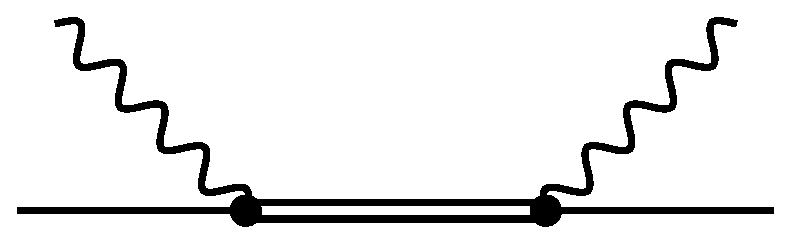
\epsfig{file=DeltaExchange.eps,width=5cm,angle=0}
\caption{Tree-level $\Delta(1232)$-exchange diagram. \label{DeltaExchange}}
\end{figure}

The counting of the $\De(1232)$ effects is done within  ``$\delta$-counting''~\cite{Pascalutsa:2003aa}, where the Delta-nucleon mass difference,
$\varDelta=M_\Delta-M$, is a light scale ($\varDelta \ll \La_\chi$) which is
substantially heavier than the pion mass ($m_\pi\ll\varDelta)$. Hence, if $p\sim m_\pi$, 
then $\mathcal{O}(p^4/\varDelta)$ is in between of $\mathcal{O}(p^3)$ and $\mathcal{O}(p^4)$. 


For the non-Born VVCS amplitudes
and polarizabilities the predictive orders are $\mathcal{O}(p^3)$ and $\mathcal{O}(p^4/\varDelta)$.
The $\mathcal{O}(p^3)$ contribution comes from the pion-nucleon ($\pi N$) loops.
We refer to it here as the LO contribution.\footnote{In the full Compton amplitude (i.e., 
including the Born term) it is, in fact, a next-to-leading-order contribution, and this is how it is referred to sometimes, e.g.~in Ref.~\cite{Lensky:2009uv}. }
The $\mathcal{O}(p^4/\varDelta)$ contribution, arising at the NLO, 
comes from the tree-level Delta-exchange ($\Delta$-exchange) graph shown in  Fig.~\ref{DeltaExchange}, and the pion-Delta ($\pi \Delta$) loops. The loop diagrams are shown in Ref.~\cite[Figs.~1 and 2]{Lensky:2014dda}.

The $\Delta$-exchange graph is described by the $\gamma^* N \Delta$ interaction in \Eqref{gammaNDeltaLag}. For the magnetic coupling, one assumes a dipole behavior to mimic the form expected from 
vector-meson dominance:
\begin{equation}
g_M\to \frac{g_M}{\big[1+\left(Q/\Lambda\right)^2\big]^2}\,,
\end{equation}
with the dipole mass $\Lambda^2=0.71$~GeV${^2}$. The inclusion of this $Q^2$ dependence is motivated by observing the importance of this form factor for the correct description of the electroproduction data \cite{Pascalutsa:2005vq}. Since electroproduction off the nucleon is directly connected with the nucleon polarizabilities via sum rules, it is understandable that a better description of the electroproduction data will lead to a better description of the $Q^2$ behavior of the polarizabilities. The effect of the dipole form factor in $g_M$ is illustrated in Fig.~\ref{Fig:alpha+beta-orders}.


A feature of the $\delta$-counting is that the characteristic momentum
$p$ distinguishes two regimes: the {\it low-energy} ($p\simeq m_\pi$) and 
{\it resonance} ($p\simeq \varDelta$) regimes. The above counting is limited to the 
low-energy regime.
Since we are interested in the low-energy expansion of the  VVCS amplitudes (i.e., $\nu=0$ with $Q^2$ finite),
we do not consider the regime where one-Delta-reducible graphs are enhanced (resonance regime).
However, going to higher $Q^2$ one does need to count the 
Delta propagators similar to the nucleon propagators, which, in turn, calls for inclusion
of $\pi \Delta$ loops with two and three Delta propagators, which have been omitted here. They are only included implicitly 
 by adjusting the isospin coefficients of the one-nucleon-reducible $\pi \Delta$-loop graphs to restore current conservation, as explained in the next section. Apart from that, $\pi \Delta$ loops have a rather mild
dependence on momenta and the missing loops are unlikely to  affect the
$Q^2$-dependence of the moments of structure functions significantly, even for $Q^2$ comparable to $\varDelta^2$. 








\subsection{Renormalization}

The calculation of the $\pi N$- and $\pi\Delta$-loop graphs is analogous to Ref.~\cite{Lensky:2009uv}, with the obvious extension to the case of a finite photon virtuality. The renormalization is also done in the exact same way; 
namely, 
subtracting the loop contribution to the Born term of the the VVCS amplitude.
The $\pi \Delta$-loop graphs
still contain divergences after this subtraction. These divergences are of higher orders, $\mathcal{O}(p^5/\varDelta^2)$ and  $\mathcal{O}(p^4)$,
and will be cancelled by the corresponding higher-order
contact terms. In practice, they are removed by taking the $\overline{\text{MS}}$ values of the divergent quantities.

As mentioned above, $\pi \Delta$-loop graphs where photons couple minimally to the Delta contain more 
than one Delta propagator and therefore should be suppressed by extra powers of $p/\varDelta$.
However, their lower-order contributions are important for electromagnetic gauge invariance and therefore for the 
renormalization procedure. In particular, the lower-order contributions of chiral loops should not affect the result of the LET~\cite{Low:1954kd, GellMann:1954kc}, and this condition is automatically satisfied by a subset of graphs if it obeys gauge invariance. The $\pi\Delta$-loop graphs, cf.\ Ref.~\cite[Fig.~2]{Lensky:2014dda}, form such a subset for the case of the neutral Delta. In reality, the Delta comes in four charge states (isospin $3/2$), thus, a 
gauge-invariant set will in addition have the higher-order graphs where the photon couples minimally to the Delta. To make the subset of $\pi\Delta$-loop graphs  gauge invariant without the higher-order graphs, we used the same procedure as in Ref.~\cite{Lensky:2009uv}. The one-particle-irreducible (1PI) graphs in Ref.~\cite[Fig.~2]{Lensky:2014dda} are computed with the correct isospin factors, i.e., summing over all charge 
states of the Delta, whereas the isospin factors for the one-particle-reducible (1PR) loop graphs are chosen such that their ratio to the isospin factors
of 1PI graphs is the same as in the neutral Delta case. This procedure automatically ensures exact gauge invariance and thus 
effectively includes the relevant contributions of the one-loop graphs with minimal coupling of photons to the Delta. If the latter graphs 
are included explicitly, the isospin factors of 1PR graphs can be restored to actual values.
The corresponding change in the values of the polarizabilities, however, is of higher order than what we consider in this work.





\subsection{Uncertainty estimate}

To estimate the uncertainties of our NLO predictions, we define the running expansion parameter
\begin{align}
 \tilde{\delta}(Q^2) = \sqrt{ \left(\frac{\varDelta}{M_N}\right)^2 + \left(\frac{Q^2}{2 M_N \varDelta}\right)^2 },\eqlab{dtilde}
\end{align}
such that the N$^2$LO is expected to be of relative size $\tilde{\delta}^2$ \cite{Pascalutsa:2005vq}.
To estimate the uncertainty of a polarizability $P(Q^2)$ due to the neglected higher-order terms in the
chiral expansion, we separate that polarizability into the static piece
$P(0)$ and the $Q^2$-dependent remainder $P(Q^2)-P(0)$. The uncertainty of $P(Q^2)$ is obtained adding the
estimates for these two parts in quadrature:
\beq
\Delta P(Q^2)= \sqrt{\tilde \delta^4(0) P(0)^2 +\tilde \delta^4(Q^2) \left[P(Q^2)-P(0)\right]^2},
\eeq
The uncertainties in the values of the parameters have a much smaller impact compared to the truncation
uncertainty and are therefore neglected.





\section{Results and discussion}

In this section, we present the B$\chi$PT predictions for the moments of the nucleon structure functions, obtained from the LEX of the VVCS amplitudes. We also consider the proton subtraction function $\ol{T}_1(0,Q^2)$. In addition to providing the full NLO results, we also analyse the individual contributions from the $\pi N$ loops, the $\Delta$ exchange, and the $\pi \Delta$ loops. 





%\section{Scalar Polarizabilities}
\label{Sec:Scalar-Pol}

\subsection{\boldmath{$M_1^{(2)}(Q^2)$} --- the generalized Baldin sum rule}


\begin{figure}[hbt]
\begin{center}
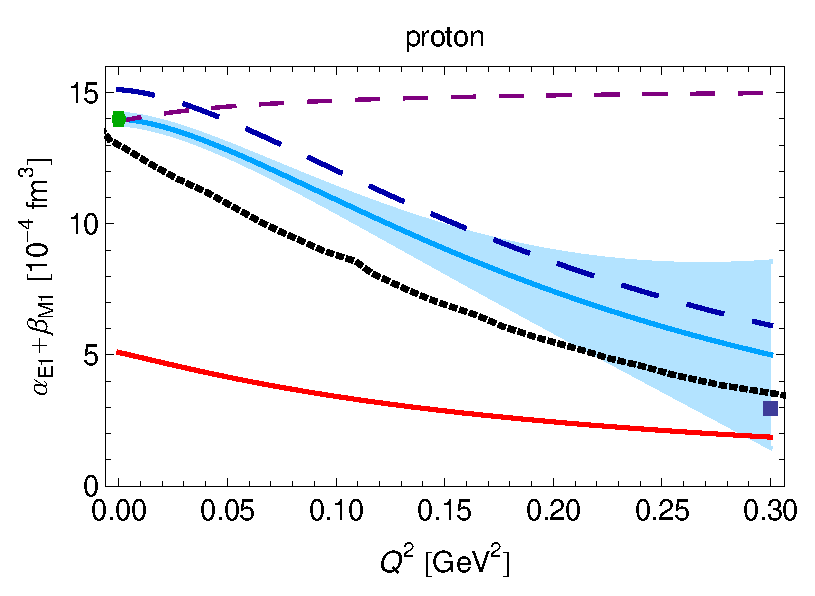
\epsfig{file=alpha+beta_p-Dip.eps,width=0.49\textwidth,angle=0} 
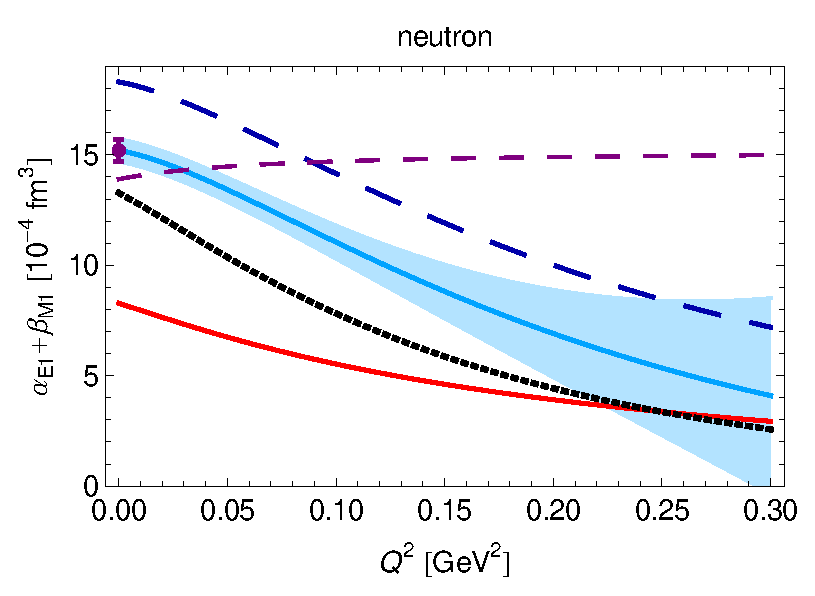
\epsfig{file=alpha+beta_n-Dip.eps,width=0.49\textwidth,angle=0} \\
\vspace{0.5cm}
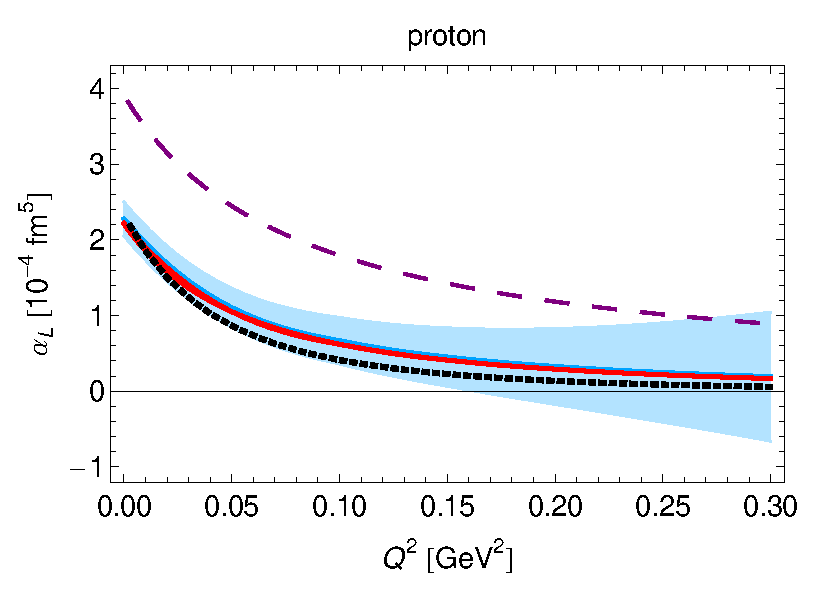
\epsfig{file=alphaL_p.eps,width=0.49\textwidth,angle=0}
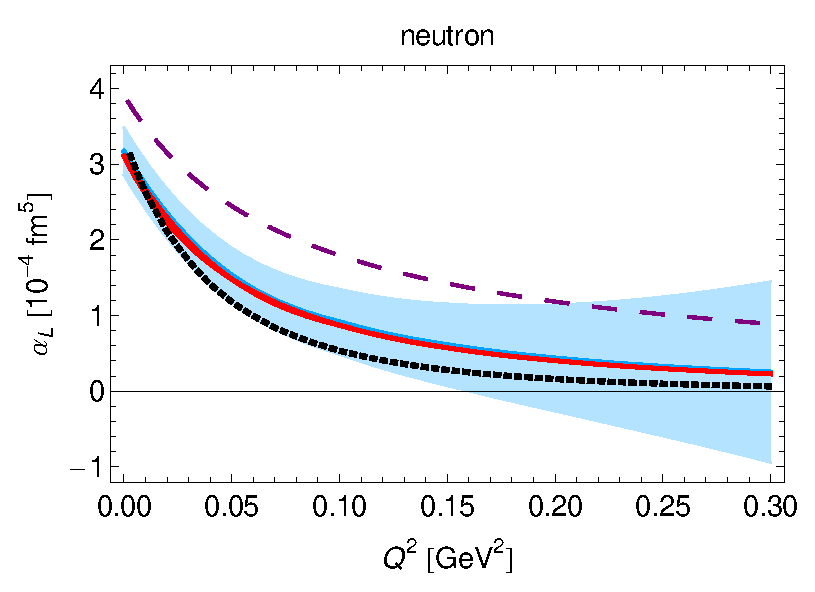
\epsfig{file=alphaL_n.eps,width=0.49\textwidth,angle=0}
\caption{Upper panel: Sum of electric and magnetic dipole polarizabilities for the proton (left) and neutron (right) as function of $Q^2$.  
The result of this work, including the fit of the static value to the Baldin sum rule, is shown by the blue solid line, with the blue band representing the uncertainty due to higher-order effects. The blue long-dashed line corresponds to the pure NLO B$\chi$PT prediction without fit to the Baldin sum rule.
The red line represents the LO B$\chi$PT result, while the purple dashed line is the LO HB limit~\cite{Nevado:2007dd}.
The black dotted line is the MAID model prediction~\cite{Drechsel:2000ct,Drechsel:1998hk,private-Lothar};  for the proton we use the updated estimate from Ref.~\cite{Drechsel:2002ar} that include the $\pi, \eta, \pi\pi$ channels.
At $Q^2=0$~GeV$^2$, we show the Baldin sum rule value for the proton (green dot)~\cite{Gryniuk:2015aa} and neutron (purple dot)~\cite{Levchuk:1999zy}.
 For the proton, the $Q^2=0.3$~GeV$^2$ point (blue square) is the empirical evaluation of Ref.~\cite{Liang:2004tk}. Lower panel: Longitudinal polarizability. Note that the LO and NLO B$\chi$PT prediction of this work nearly coincide. 
 \label{Fig:alpha+betaplot}}
\end{center}
\end{figure}



%\begin{figure}[hbt]
%\begin{center}
%\epsfig{file=BSRp.pdf,width=0.49\textwidth,angle=0} \hspace{0.5cm}
%\epsfig{file=BSRn.pdf,width=0.49\textwidth,angle=0} 
%\caption{{\color{red} A FIRST VERSION OF THE NEW PLOTS TO TEST THE LOOKS --- BALDIN SUM RULE FITTED AT $Q^2=0$, NOT ALL CURVES YET INCLUDED.}\\
%Sum of electric and magnetic dipole polarizabilities, $\alpha_{E1}(Q^2)+\beta_{M1}(Q^2)$, for the proton ($p$) and neutron ($n$) as function of $Q^2$.  
%The result of this work is shown by the blue solid line and the blue band.
%The red line represents the LO B$\chi$PT result, while the blue dashed line is the LO HB limit~\cite{Nevado:2007dd}.
%The black dotted line is the MAID model prediction~\cite{Drechsel:2000ct,Drechsel:1998hk,private-Lothar}; note that for the proton we use the updated estimate from Ref.~\cite{Drechsel:2002ar} obtained using the $\pi+\eta+\pi\pi$ channels.
%At $Q^2=0$~GeV$^2$, we show Baldin sum rule evaluations for the proton (green dot)~\cite{Gryniuk:2015aa} and neutron (purple dot)~\cite{Babusci:1997ij}.
% The $Q^2=0.3$~GeV$^2$ point (blue dot) is an evaluation of the generalized Baldin sum rule \cite{Liang:2004tk}.
% \label{Fig:alpha+betaplot}}
%\end{center}
%\end{figure}

\begin{figure}
\begin{center}
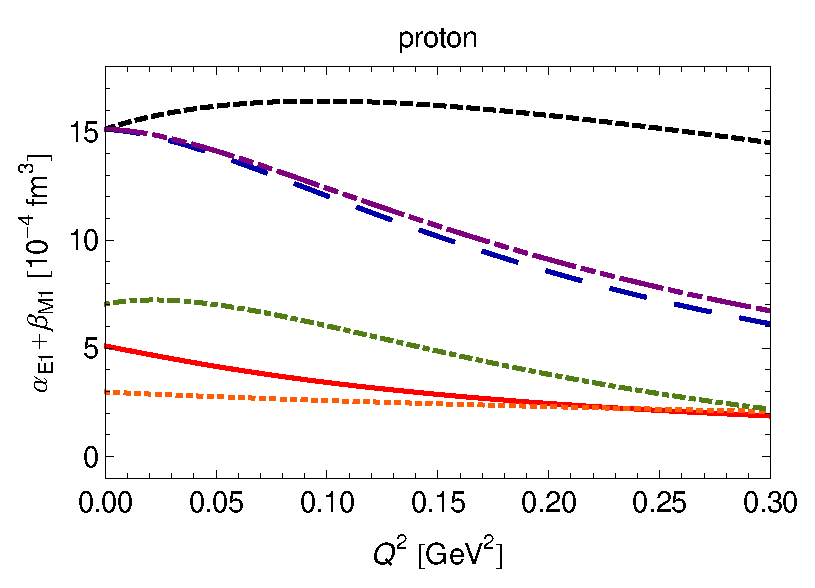
\epsfig{file=alpha+beta_p-orders-Dip.eps,width=0.49\textwidth,angle=0}
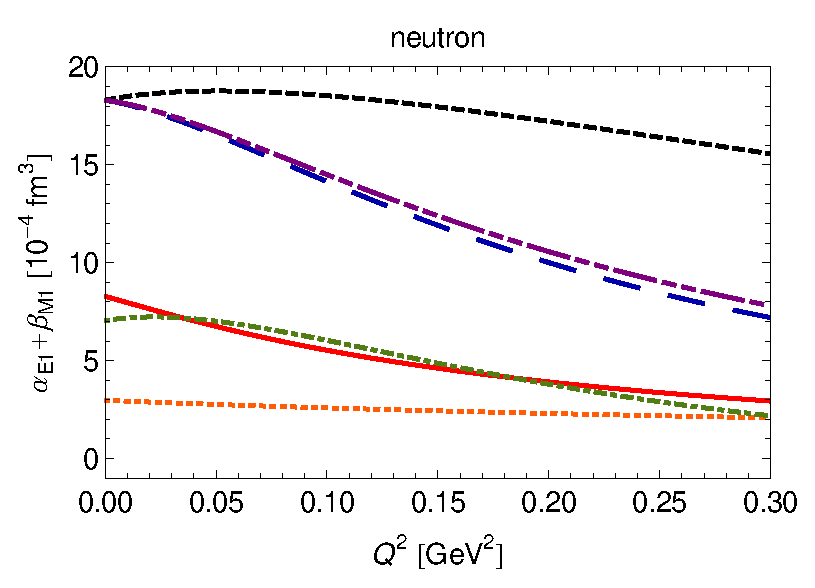
\epsfig{file=alpha+beta_n-orders-Dip.eps,width=0.49\textwidth,angle=0} \\ \vspace{0.5cm}
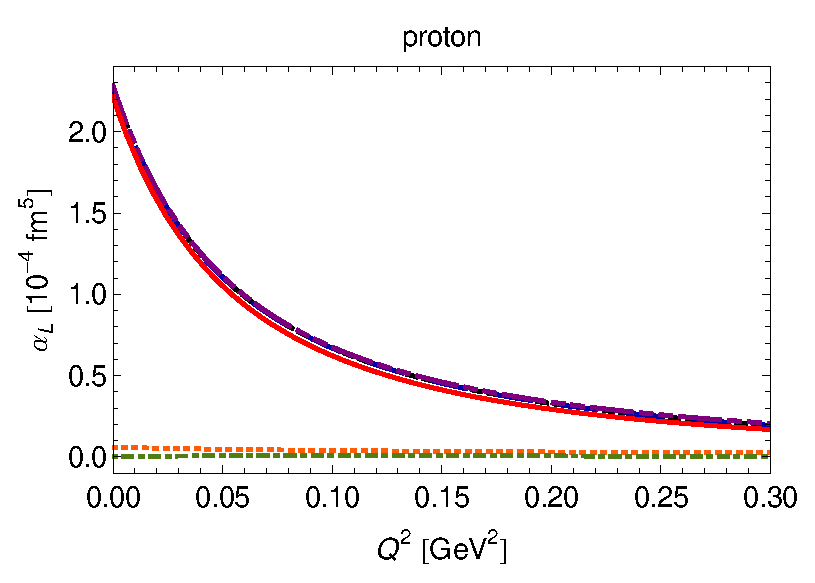
\epsfig{file=alphaL_p-orders-Dip.eps,width=0.49\textwidth,angle=0}
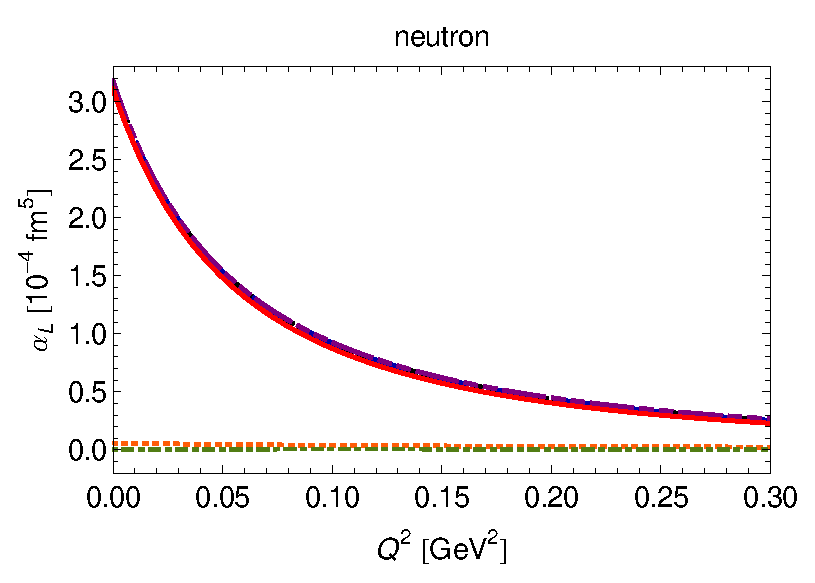
\epsfig{file=alphaL_n-orders-Dip.eps,width=0.49\textwidth,angle=0} 
\caption{\small{Contributions of the different orders to the chiral predictions of $[\alpha_{E1}+\beta_{M1}](Q^2)$ \{upper panel\} and $\alpha_L(Q^2)$ \{lower panel\}. Red solid line: $\pi N$-loop contribution, green dot-dashed line: $\Delta$-exchange contribution, orange dotted line: $\pi \Delta$-loop contribution, blue long-dashed line: total result, purple dot-dot-dashed line: total result without $g_C$ contribution, black short-dashed line: total result without $g_M$ dipole.}\label{Fig:alpha+beta-orders}}
\end{center}
\end{figure}

The electric and magnetic dipole polarizabilities, $\alpha_{E1}(Q^2)$ and $\beta_{M1}(Q^2)$, encode information about the dipole response of the nucleon to an electromagnetic field. For finite momentum transfers, the sum of the dipole polarizabilities is given by the generalized Baldin sum rule:
\beq
[\alpha_{E1}+\beta_{M1}] (Q^2)= \frac{1}{2 \pi^2} \int_{\nu_0}^\infty \! \dd\nu\,\sqrt{1+\frac{Q^2}{\nu^2}}\, \frac{\sigma_T (\nu,Q^2)}{\nu^2} =\frac{8 \al M_N}{Q^4}\int_0^{x_0}\!\dd x\, x \,F_1(x,Q^2),\label{Eq:alpha+betaQ2}
\eeq
where $\nu_0$ is the lowest inelastic threshold, in this case the one-pion production threshold $\nu_0=m_\pi + (m_\pi^2+Q^2)/2M_N$, and $x_0=Q^2/2M_N \nu_0$.
%The information encoded in these polarizabilities is of major interest to extract the proton radius from the measurement of the $\mu$H Lamb shift \cite{Birse:2012eb,Alarcon:2013cba,Carlson:2011zd,Nevado:2007dd,Peset:2014yha,Hagelstein:2017cbl}, since they provide the structure corrections needed for an accurate extraction of the proton radius.
The electric and magnetic dipole polarizabilities of the nucleon enter the nucleon-structure contributions
to the Lamb shift of $\mu$H and other muonic atoms \cite{Bernabeu:1982qy,Pachucki:1996zza,Carlson:2011zd,Alarcon:2013cba}, and thus
are of major interest for an accurate extraction of the nuclear charge radii.

Our B$\chi$PT predictions for $\alpha_{E1}+\beta_{M1}$ are shown in Fig.~\ref{Fig:alpha+betaplot}, both for the proton
and the neutron, up to photon virtualities of $0.3$~GeV$^2$. We show our complete NLO results, which include the $\pi N$-loop, the $\Delta$-exchange and the $\pi \Delta$-loop contributions. In order to illustrate the effect of the Delta in these predictions, we also plot the LO $\pi N$-loop contribution
separately. We compare our results for the $Q^2$
evolution with the LO HB$\chi$PT predictions~\cite{Nevado:2007dd} and the MAID model predictions~\cite{Drechsel:2000ct,Drechsel:1998hk}. The latter are based on the generalized Baldin sum rule~\eqref{Eq:alpha+betaQ2} evaluated with ($\pi+\eta+\pi \pi$) photoproduction
cross sections~\cite{Drechsel:2002ar}. 
The data point are also evaluations of the (generalized) Baldin sum rule \cite{Liang:2004tk,Gryniuk:2015aa,Babusci:1997ij}. One can see that the B$\chi$PT predictions seem to systematically overestimate the MAID model in the $Q^2$ range shown here. 

The LO HB results seem to agree with the empirical values at the real-photon point~\cite{Babusci:1997ij}
both for the proton and the neutron. However, they do not fall off with increasing $Q^2$ in contrast to the B$\chi$PT predictions.
This asymptotic behavior is the reason for the large proton-polarizability effect on the muonic-hydrogen Lamb shift found within HB$\chi$PT \cite{Nevado:2007dd,Peset:2014yha}, much larger than the phenomenological value. As shown in Ref.~\cite{Alarcon:2013cba,Lensky:2017bwi}, this issue is solved within the relativistic formulation, which gives a result closer to calculations based on the dispersive approach.


The static dipole polarizabilities $\alpha_{E1}$ and $\beta_{M1}$ have been  studied  within both the HB  and
the B$\chi$PT. While  HB$\chi$PT gives results
remarkably close to the experimental determinations already at LO \cite{Bernard:1995dp},
the contribution of the $\Delta(1232)$ is harder to accommodate in this framework~\cite{Hemmert:1996rw}. In contrast to that, LO  B$\chi$PT \cite{Bernard:1991rq,Bernard:1991ru}
yields smaller values for the sum of dipole polarizabilities, in disagreement with the empirically extracted values based on evaluations of the Baldin sum rule with modern photoabsorption data~\cite{Babusci:1997ij,Olm01,Gryniuk:2015aa}. However, the NLO contributions from $\Delta$ exchange and $\pi\Delta$ loops improve the situation \cite{Lensky:2009uv,Lensky:2015awa}.
In the case of the proton, they bring the B$\chi$PT result in agreement with the experimental extraction, while for the neutron the total result is slightly bigger. The $\Delta(1232)$ contributions are therefore naturally accommodated in  B$\chi$PT but not in HB$\chi$PT.
%{\color{blue} We may need to give newer references here.}

The B$\chi$PT contributions from $\pi N$ loops, $\Delta$ exchange and $\pi \Delta$ loops to the static polarizabilities are, in that order and in the usual units of $10^{-4}$~fm$^3$:
\begin{align}
\alpha_{E1}^{(p)}+\beta_{M1}^{(p)}=15.12(1.48) \approx 5.10+7.04+2.98, \label{Eq:alpha+betaProtonRealPoint}\\
\alpha_{E1}^{(n)}+\beta_{M1}^{(n)} =18.30(1.79)\approx 8.28+7.04+2.98. \label{Eq:alpha+betaNeutronRealPoint}
\end{align}
The corresponding individual contributions to the $Q^2$-dependent generalized polarizabilities are shown in Fig.~\ref{Fig:alpha+beta-orders}.
For the proton, the dominant contribution in the studied $Q^2$ range is that of the $\Delta$ exchange, while for the neutron the $\pi N$-loop and $\Delta$-exchange contributions are of roughly the same size.
The importance of the Delta is related to the fact that the nucleon-to-Delta transition, which is dominantly of magnetic dipole type, gives a huge contribution to $\beta_{M1}$. 




In addition to their static values, it is also interesting to investigate the slopes of the polarizabilities at the real-photon point. Decomposing the results as before, we observe that B$\chi$PT predicts large contributions to the slopes both from $\pi N$ loops and $\Delta$ exchange. The $Q^2$ dependence generated by $\pi \Delta$ loops, on the other hand, is negligible,
as can be clearly seen from Fig.~\ref{Fig:alpha+beta-orders}. The numerical values for the individual contributions to the slopes are, in units of $10^{-4}$~fm$^5$:
\bea
\left.\frac{\dd(\alpha_{E1}^{(p)} + \beta_{M1}^{(p)}) (Q^2)}{\dd Q^2}\right|_{Q^2=0}&=&-0.19(6)\approx -0.74  + 0.74-0.20 ,\\
\left.\frac{\dd(\alpha_{E1}^{(n)} + \beta_{M1}^{(n)}) (Q^2)}{\dd Q^2}\right|_{Q^2=0}&=& -0.68(21)\approx-1.22  +0.74-0.20.
\eea
 The dipole form factor in the magnetic coupling $g_M$ generates the $Q^2$ fall-off of the dipole polarizabilities, cf.\ Fig.~\ref{Fig:alpha+beta-orders}, which is also observed
in parametrizations of experimental cross sections~\cite{Hall:2014lea}. 
Due to cancellations between the $\pi N$-loop and the $\Delta$-exchange contributions,
 the dipole also crucially affects the overall sign of the slope, as can be seen in Fig.~\ref{Fig:alpha+beta-orders}. Note that due to these cancellations we estimate its relative error
 of the slope by $\tilde{\delta}$ instead of $\tilde{\delta}^2$.


Evaluating the Baldin sum rule radius, 
\begin{align}\label{Eq:r2alphabetaDef}
r_{\alpha+\beta}^2\equiv \frac{-6}{(\alpha_{E1}+\beta_{M1})}\left.\frac{\dd}{\dd Q^2}[\alpha_{E1}+\beta_{M1}](Q^2)\right|_{Q^2=0},
\end{align}
we obtain $r^{(p)}_{\alpha+\beta}= 0.28(9)$~fm and $r^{(n)}_{\alpha+\beta}=0.47(15)$~fm, 
where we estimated the relative error to be $\tilde{\delta}$. This can be compared to the empirical $r^{(p)}_{\alpha+\beta}=0.98(5)$~fm~\cite{Hall:2014lea}. Due to the big impact of the $Q^2$ dependence in $g_M$, our result is very different from the one in Ref.~\cite{Hall:2014lea}.
Fortunately, this effect is smaller for the polarizabilities.




\subsection{\boldmath{$\alpha_L (Q^2)$} --- the longitudinal polarizability}




The longitudinal polarizability,
\beq
\alpha_L (Q^2)= \frac{1}{2 \pi^2} \int_{\nu_0}^\infty\! \dd\nu\,\sqrt{1+\frac{Q^2}{\nu^{2}}}\,            \frac{\sigma_L (\nu,Q^2)}{Q^2\, \nu^{2}} = \frac{4 \al M_N}{Q^6}\int_0^{x_0}\! \dd x \, F_L(x,Q^2),\label{Eq:alphaLQ2}
\eeq
with
\beq
F_L(x,Q^2)=-2xF_1(x,Q^2)+\left[1+\frac{4M_N^2 x^2}{Q^2}\right]F_2(x,Q^2),\nn
\eeq
provides information about the internal structure of the nucleon responding to longitudinaly polarized photons. 
It contributes to $T_2(\nu,Q^2)$ at $\mathcal{O}(Q^4)$, and therefore, is a  subleading structure correction to the (muonic-)hydrogen Lamb shift.

Our B$\chi$PT prediction for $\alpha_L(Q^2)$ is shown in Fig.~\ref{Fig:alpha+betaplot}, 
where we compare our results, with and without the Delta contributions, with the MAID model predictions~\cite{Drechsel:2000ct,Drechsel:1998hk,Drechsel:2002ar,private-Lothar} and the HB limit of the $\pi N$-loop contribution. One can see that the Delta plays a negligible role in the low-$Q^2$ evolution of $\alpha_L$, which in the B$\chi$PT approach is dominated by $\pi N$ loops.
Our results run very close to the MAID curves, with small discrepancies in the intermediate $Q^2$ region.
At higher virtualities, these discrepancies decrease.
The HB approach, on the other hand, seems to systematically overestimate the value of $\alpha_L$ in the considered $Q^2$ range. 
This relatively big mismatch, very similar to the discrepancy observed in HB calculations of $\delta_{LT}^{(n)}$, can be traced back to the slow convergence of the $1/M_N$ expansion, as one can see from the analytic expression for the $\pi N$-loop contribution to $\alpha_L(Q^2=0)$ given in  Appendix~\ref{App:Polarizabilities}.  As in the case of $\delta_{LT}^{(n)}$, this systematic deviation is cured in the relativistic formulation. 

For the static values of $\alpha_L$,
we obtain the following contributions from $\pi N$ loops,  $\Delta$ exchange and $\pi\Delta$ loops, in units of $10^{-4}$~fm$^5$:
\begin{align}
\alpha^{(p)}_L=2.28(22)\approx 2.22+ 0.00+  0.06, \\
\alpha^{(n)}_L= 3.17(31)\approx 3.11 + 0.00+ 0.06.
\end{align}
For the slopes at $Q^2=0$, we find, in units of $10^{-4}$~fm$^7$:
\begin{align}
\left.\frac{\dd\alpha^{(p)}_L (Q^2)}{\dd Q^2}\right|_{Q^2=0}&=-1.63(16)\approx  -1.62 + 0.01 - 0.01  ,  \\
\left.\frac{\dd\alpha^{(n)}_L (Q^2)}{\dd Q^2}\right|_{Q^2=0}&= -2.25(22)\approx -2.24 + 0.01 - 0.01.
\end{align}
 The corresponding individual contributions to the $Q^2$ dependence
of $\alpha_L(Q^2)$ are demonstrated in Fig.~\ref{Fig:alpha+beta-orders}. One again notices
that  $\Delta$ exchange and  $\pi \Delta$ loops give negligible contributions in this $Q^2$ range, with the $\Delta$-exchange contribution being even smaller than the $\pi \Delta$-loop contribution. 
The latter feature is explained by the fact that the magnetic coupling $g_M$ does not contribute to $\al_L$.

\subsection{\boldmath{$M^{(4)}_1(Q^2)$} --- the fourth-order Baldin sum rule}

\bea
 M_1^{(4)}(Q^2)&=& 
\frac{1}{2 \pi^2} \, \int_{\nu_0}^{\infty}\, \mathrm{d}\nu \,\sqrt{1+\frac{Q^2}{\nu^{2}}}\, \frac{\sigma_T(\nu)}{\nu^{4} }\\
&=&\frac{32 \al M_N^3}{Q^8}\int_0^{x_0}\!\dd x\, x^3 \,F_1(x,Q^2) \nn, 
\eea

In the real photon limit, this moment is related to the sum of dispersive and quadrupole polarizabilities:
\beq
M_1^{(4)}(0)=\alpha_{E1 \nu} + \beta_{M1 \nu} + \frac{1}{12} (\alpha_{E2} + \beta_{M2}) .
\eeq

For the static values of $M_1^{(4)}$,
we obtain the following contributions from $\pi N$ loops,  $\Delta$ exchange and $\pi\Delta$ loops, in units of $10^{-4}$~fm$^5$:
\begin{align}
M_1^{(4)(p)}=6.00(59)\approx2.95+2.92+0.13, \\
M_1^{(4)(n)}=7.30(72) \approx 4.26+2.92+0.13.
\end{align}
For the slopes at $Q^2=0$, we find, in units of $10^{-4}$~fm$^7$:
\begin{align}
\left.\frac{\dd M_1^{(4)(p)} (Q^2)}{\dd Q^2}\right|_{Q^2=0}&=-1.38(14)\approx -1.16-0.20-0.02  ,  \\
\left.\frac{\dd M_1^{(4)(n)} (Q^2)}{\dd Q^2}\right|_{Q^2=0}&=-1.96(19) \approx -1.73-0.20-0.02.
\end{align}
 The corresponding individual contributions to the $Q^2$ dependence
of $M_1^{(4)}(Q^2)$ are demonstrated in Fig.~\ref{Fig:M14-orders}.

\begin{figure}[hbt]
\begin{center}
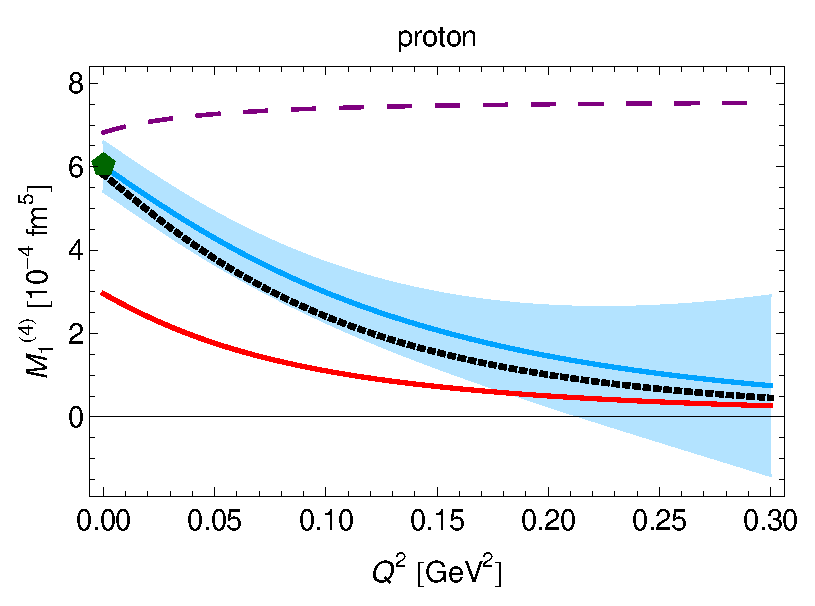
\epsfig{file=M14_p-Dip.eps,width=0.49\textwidth,angle=0} 
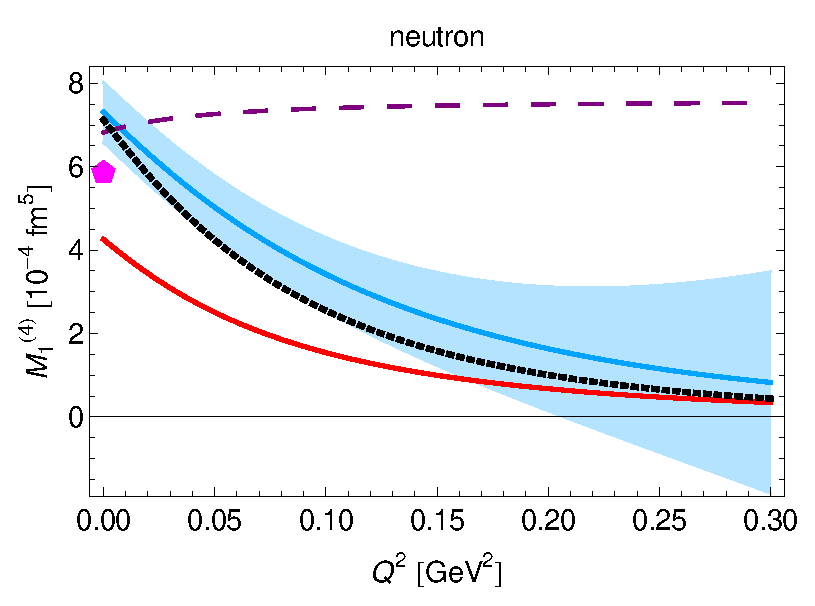
\epsfig{file=M14_n-Dip.eps,width=0.49\textwidth,angle=0} 
\caption{
The fourth-order generalized Baldin sum rule for the proton and neutron  as function of $Q^2$.  
The result of this work is shown by the blue solid line and the blue band.
The red line represents the LO B$\chi$PT result, while the purple dashed line is the LO HB limit~\cite{Nevado:2007dd}.
The black dotted line is the MAID model prediction~\cite{Drechsel:2000ct,Drechsel:1998hk,private-Lothar}.
At $Q^2=0$~GeV$^2$, we show the fourth-order Baldin sum rule evaluations for the proton (dark green pentagon)~\cite{Gryniuk:2015aa} and neutron (magenta pentagon)~\cite{Schroder:1977sn}.
 \label{Fig:M14plot}}
\end{center}
\end{figure}

\begin{figure}
\begin{center}
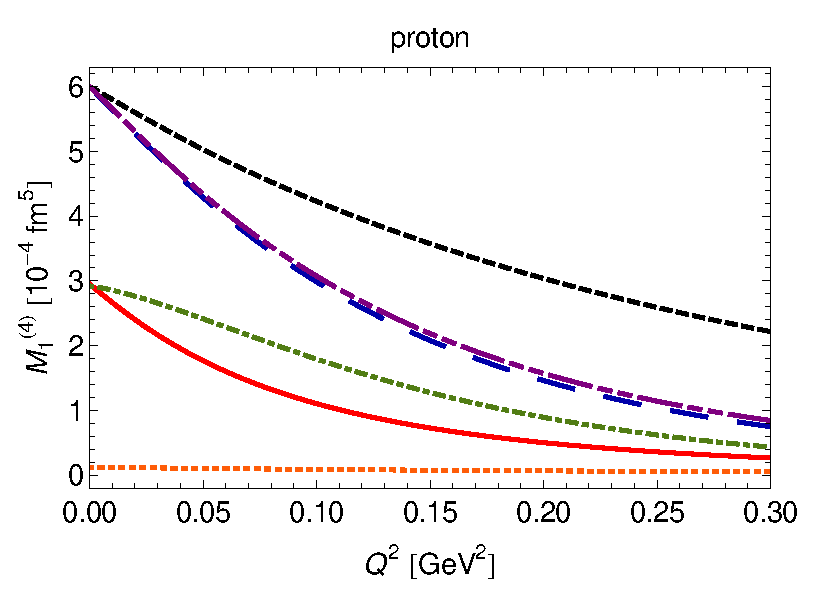
\epsfig{file=M14p-orders-Dip.eps,width=0.49\textwidth,angle=0}
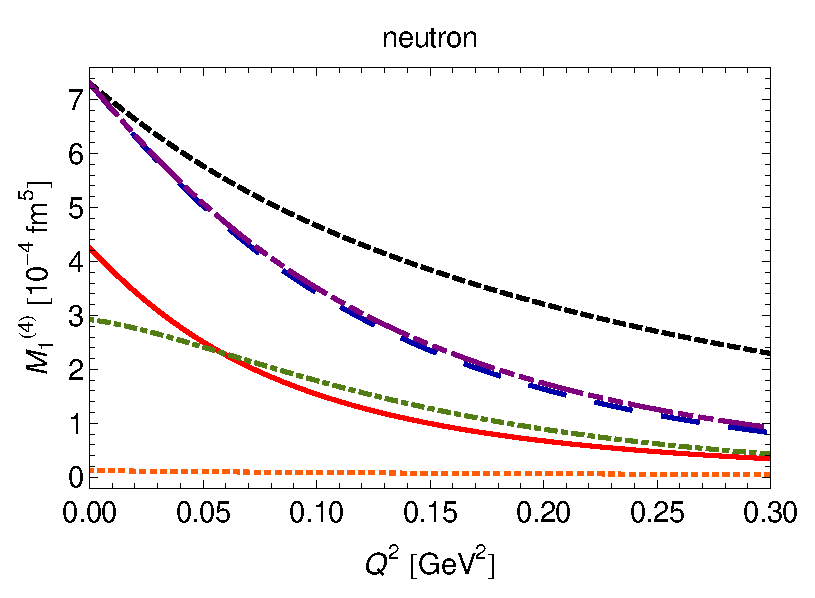
\epsfig{file=M14n-orders-Dip.eps,width=0.49\textwidth,angle=0} 
\caption{\small{Contributions of the different orders to the chiral prediction of $M_1^{(4)}(Q^2)$. Red solid line: $\pi N$-loop contribution, green dot-dashed line: $\Delta$-exchange contribution, orange dotted line: $\pi \Delta$-loop contribution, blue long-dashed line: total result, purple dot-dot-dashed line: total result without $g_C$ contribution, black short-dashed line: total result without $g_M$ dipole.}\label{Fig:M14-orders}}
\end{center}
\end{figure}

\subsection{\boldmath{$M^{(1)}_2(Q^2)$} --- the first moment of $F_2(x,Q^2)$}

\bea
M^{(1)}_2(Q^2)  &=& \frac{1}{2 \pi^2}  \int_{\nu_0}^{\infty}\, 
\frac{\mathrm{d}\nu}{\nu}  
\frac{1}{\sqrt{\nu^{2}+Q^2}}\left[ \frac{}{} \sigma_T(\nu, Q^2 ) +  \sigma_L(\nu, Q^2 )\right],   
\label{eq:m21}\\
&=&\frac{4 \al M_N}{ Q^4}\,\int_{0}^{x_0} \mathrm{d}x  \,F_2(x,\,Q^2) 
\nn 
\eea 

%For the static values ,
%we obtain the following contributions from $\pi N$ loops,  $\Delta$ exchange and $\pi\Delta$ loops, in units of $10^{-4}$~fm$^3$:
%\begin{align}
%M_2^{(1)(p)}&=15.12(1.48)\approx  5.10+7.04+2.98 , \\
%M_2^{(1)(n)}= &=18.30(1.79) \approx 8.28 +7.04+2.98.
%\end{align}
For the slopes of $M_2^{(1)}$ at $Q^2=0$, we find, in units of $10^{-4}$~fm$^5$:
\begin{align}
\left.\frac{\dd M_2^{(1)(p)} (Q^2)}{\dd Q^2}\right|_{Q^2=0}&= -3.92(38)\approx -1.47-2.18-0.26 ,  \\
\left.\frac{\dd M_2^{(1)(n)} (Q^2)}{\dd Q^2}\right|_{Q^2=0}&=-4.81(47) \approx -2.37-2.18-0.26 .
\end{align}
 The corresponding individual contributions to the $Q^2$ dependence
of $M_2^{(1)}(Q^2)$ are demonstrated in Fig.~\ref{Fig:M21-orders}.

\begin{figure}[hbt]
\begin{center}
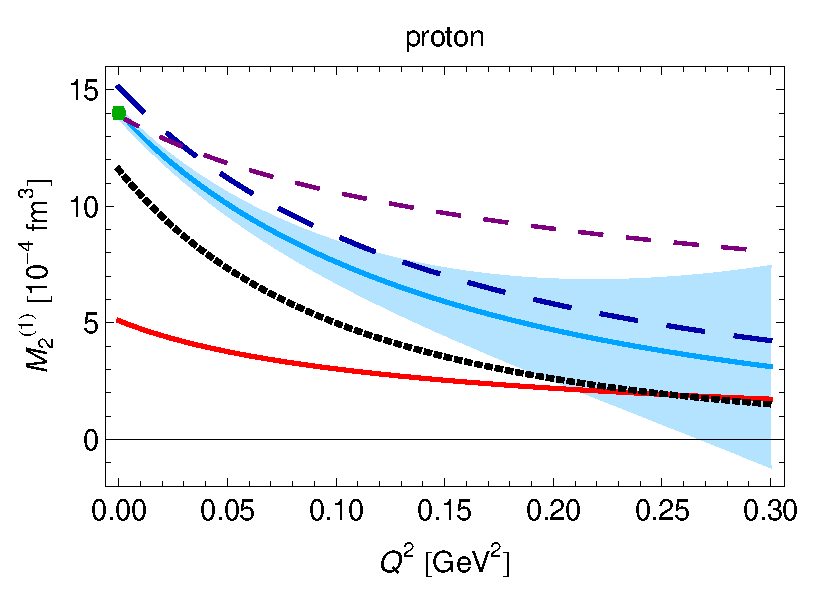
\epsfig{file=M21_p-Dip.eps,width=0.49\textwidth,angle=0} 
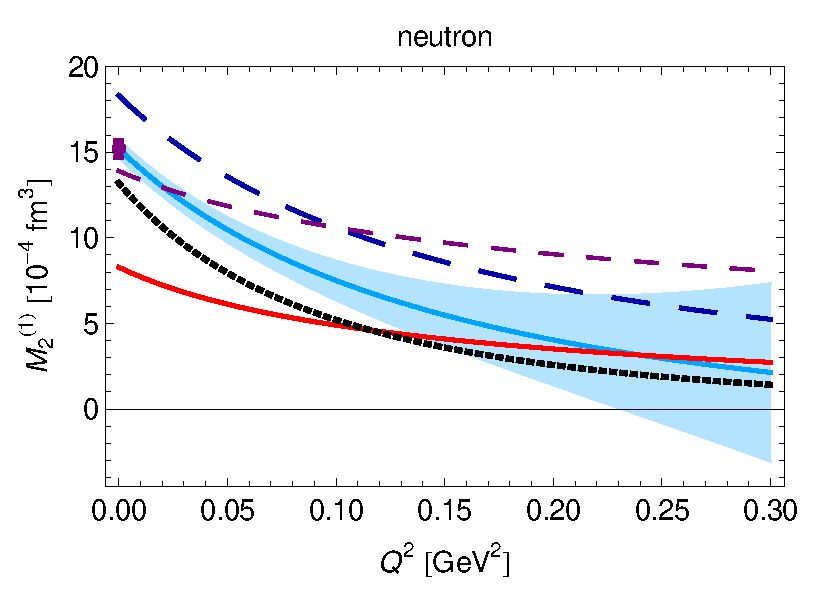
\epsfig{file=M21_n-Dip.eps,width=0.49\textwidth,angle=0}
\caption{
The first moment of the structure function $F_2(x,Q^2)$ for the proton ($p$) and neutron ($n$) as function of $Q^2$.  
The result of this work including the fit of the static value to the Baldin sum rule is shown by the blue solid line and the blue band, while the blue long-dashed line corresponds to the pure NLO B$\chi$PT prediction without fit to the Baldin sum rule.
The red line represents the LO B$\chi$PT result, while the purple dashed line is the LO HB limit~\cite{Nevado:2007dd}.
The black dotted line is the MAID model prediction~\cite{Drechsel:2000ct,Drechsel:1998hk,private-Lothar}.
At $Q^2=0$~GeV$^2$, we show Baldin sum rule evaluations for the proton (green dot)~\cite{Gryniuk:2015aa} and neutron (purple dot)~\cite{Levchuk:1999zy}.
 \label{Fig:M21plot}}
\end{center}
\end{figure}

\begin{figure}
\begin{center}
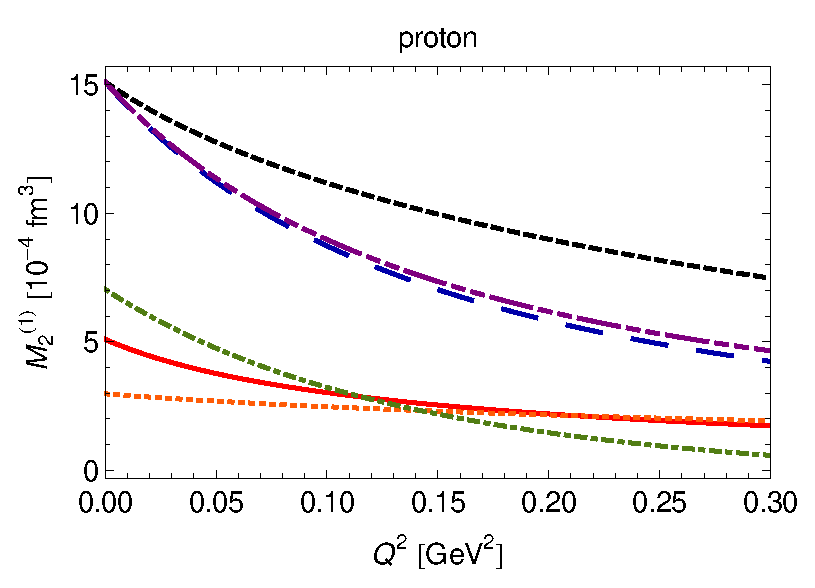
\epsfig{file=M21p-orders-Dip.eps,width=0.49\textwidth,angle=0}
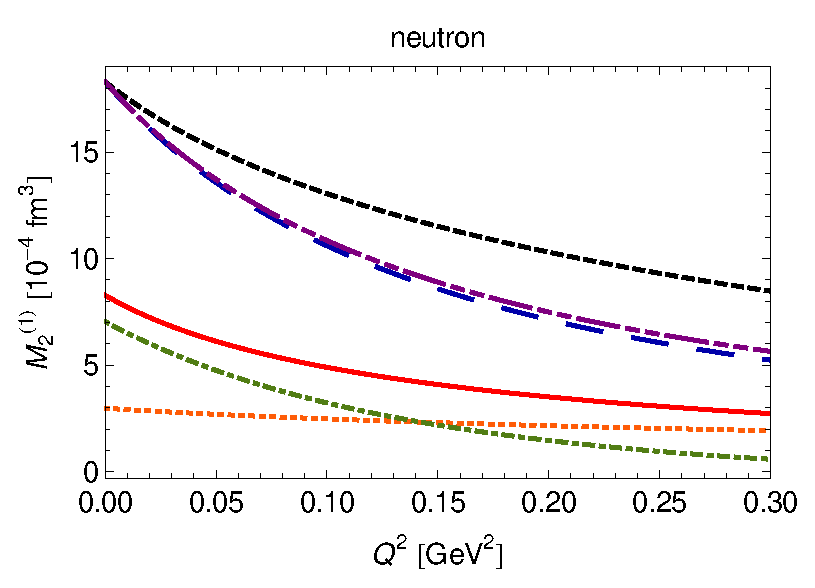
\epsfig{file=M21n-orders-Dip.eps,width=0.49\textwidth,angle=0} 
\caption{\small{Contributions of the different orders to the chiral prediction of $M_2^{(1)}(Q^2)$. Red solid line: $\pi N$-loop contribution, green dot-dashed line: $\Delta$-exchange contribution, orange dotted line: $\pi \Delta$-loop contribution, blue long-dashed line: total result, purple dot-dot-dashed line: total result without $g_C$ contribution, black short-dashed line: total result without $g_M$ dipole.}\label{Fig:M21-orders}}
\end{center}
\end{figure}

\subsection{\boldmath{$T_1(0,Q^2)$} --- the subtraction function}


\begin{figure}[bt]
\begin{center}
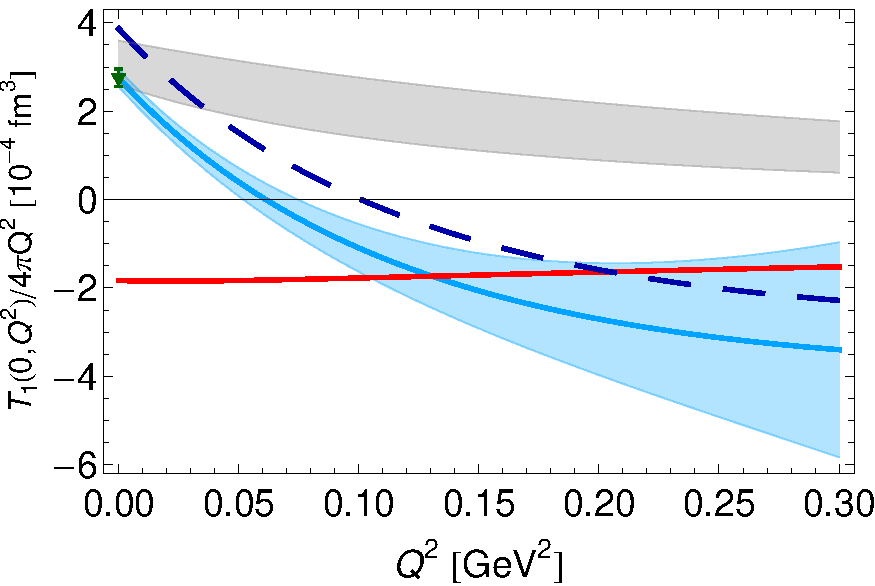
\epsfig{file=T1Rp.pdf,width=0.5\textwidth,angle=0}
\caption{The low-$Q^2$ behavior of the non-Born piece of the subtraction function $T_1(0,Q^2)/4\pi Q^2$. The result of this work, including the fit of the static value to Baldin sum rule \cite{Gryniuk:2015aa}, is shown by the blue solid line, with the blue band representing the uncertainty due to higher-order effects. The blue long-dashed line corresponds to the pure NLO B$\chi$PT prediction without fit at the real photon point to $\beta_{M1}=(2.75\pm 0.2)\times 10^{-4}~\text{fm}^3$ (dark green triangle). The red solid curve corresponds to the B$\chi$PT $\pi N$-loop contribution only, the gray band is the HB$\chi$PT calculation~\cite{Birse:2012eb}.
}
\label{fig:subtraction}
\end{center}
\end{figure}


\section{Summary and conclusions}\label{Sec:Summary}


%\begin{table}[h]
%\caption{The NLO B$\chi$PT predictions for the forward VVCS polarizabilities and their derivatives at $Q^2=0$. The contributions of the $\pi N$ loops, the $\Delta$ exchange and the $\pi\Delta$ loops are shown, together with the combined total NLO predictions.
%\label{Table:Individual-Results-Pol}}
%\begin{tabular}{cc|c|c|c|c|}
%\cline{3-6} 
%&& $\pi N$ loops & $\Delta$ exchange   & $\pi\Delta$ loops & Total \\
%\hline
%\multicolumn{1}{|c||}{$\alpha_{E1}+\beta_{M1}$} &$p$&$5.10$&$\hpm7.04$&$\hpm2.98$&$\hpm15.12(1.48)$\\
%\multicolumn{1}{|c||}{$(10^{-4}$~fm$^3)$} &$n$&$8.28$&$\hpm7.04$&$\hpm2.98$&$\hpm18.30(1.79)$\\
%\hline
%\multicolumn{1}{|c||}{$\alpha_L$}&$p$ &$2.22$&$\hpm0.00$&$\hpm0.06$&$\hpm2.28(22)$\\
%\multicolumn{1}{|c||}{$(10^{-4}$~fm$^5)$} &$n$&$3.11$&$\hpm0.00$&$\hpm0.06$&$\hpm3.17(31)$\\
%\hline
%\multicolumn{1}{|c||}{$(\alpha_{E1}+\beta_{M1})'$} &$p$&$-0.74$&$\hpm0.74$&$-0.20$&$-0.19(6)$\\
%\multicolumn{1}{|c||}{$(10^{-4}$~fm$^5)$} &$n$&$-1.22$&$\hpm0.74$&$-0.20$&$-0.68(21)$\\
%\hline
%\multicolumn{1}{|c||}{$(\alpha_L)'$}&$p$ &$-1.62$&$\hpm0.01$&$-0.01$&$-1.63(16)$\\
%\multicolumn{1}{|c||}{$(10^{-4}$~fm$^7)$} &$n$&$-2.24$&$\hpm0.01$&$-0.01$&$-2.25(22)$\\
%\hline
%\end{tabular}
%\end{table}






%\begin{table}[h]
%\caption{The NLO B$\chi$PT predictions for the forward VVCS polarizabilities at $Q^2=0$, compared with the available empirical information. Where the reference is not given, the empirical number is provided by the MAID analysis \cite{Drechsel:2000ct,MAID} with unspecified uncertainty.
%\label{Table:Results-Pol}}
%\begin{tabular}{c|c|c||c|c|}
%\cline{2-5} 
%&  \multicolumn{2}{|c||}{ Proton} & 
%\multicolumn{2}{|c|}{Neutron} \\
%\cline{2-5} 
%  & \, This work \, & Empirical   & \, This work\, & \,\,Empirical\,\, \\
%\hline
%\multicolumn{1}{|c|}{$\alpha_{E1}+\beta_{M1}$} &$\hpm15.12(1.48)$ & $13.8(4)$ &$18.30(1.79)$  &$14.40(66)$\\
%\multicolumn{1}{|c|}{$(10^{-4}$~fm$^3)$} & & Ref.~\cite{Olm01}& &Ref.~\cite{Babusci:1997ij}\\
%\hline
%\multicolumn{1}{|c|}{$\alpha_L$} &$\hpm2.28(22)$ & $2.32$ & $3.17(31)$  & $3.32$\\
%\multicolumn{1}{|c|}{$(10^{-4}$~fm$^5)$} &&[MAID]&&[MAID]\\
%\hline
%\end{tabular}
%\end{table}



In this article, we have computed a NLO parameter-free prediction of the scalar polarizabilities, as well as some other moments of the proton and neutron unpolarized structure functions for finite $Q^2$ in covariant B$\chi$PT. 
We calculated the VVCS amplitudes at N$^2$LO including explicitly the contribution of the $\Delta(1232)$ as an intermediate state with a dipole form factor for its magnetic coupling. The later turns out to be very important in the descriptions of the sum of electric and magnetic dipole polarizabilities $\alpha_{E1}+\beta_{M1}$, which indicates the importance of including vector-meson exchanges in $\chi$PT to account properly for the $Q^2$ behavior of the polarizabilities. We found that the Delta plays a fundamental role in the description of the $Q^2$ dependence of $\alpha_{E1}+\beta_{M1}$, but basically no role in the longitudinal polarizability $\alpha_L$. While the $\pi\Delta$ loops are relevant for $\alpha_{E1}+\beta_{M1}$, the Coulomb coupling $g_C$ has a only a small effect.

In general, we obtain a good description of the $Q^2$ evolution of the polarizabilities and the moments of the unpolarized structure functions, improving the previous $\chi$PT predictions.
In this regard, we compared our calculation to the HB approach \cite{Nevado:2007dd}, as well as to the MAID model prediction \cite{MAID}. 
It is shown that in our approach we obtain results which are closer to  MAID than the HB calculation.

We also proved the validity of the sum rules for $\alpha_{E1}+\beta_{M1}$ and $\alpha_L$ at LO in $\chi$PT for arbitrary $Q^2$:
Evaluating the sum rules with the $\mathcal{O}(p)$  pion electroproduction cross sections, we were able to reproduce the $\mathcal{O}(p^3)$ results for the polarizabilities and moments obtained directly from forward VVCS in covariant $\chi$PT.
We give analytic expressions for the relativistic predictions of the $\pi N$-loop and $\Delta$-exchange contributions to the static polarizabilities and moments, as well as their slopes, see Appendix~\ref{App:PolarizabilitiesAll}.
For some polarizabilities, such expansions are given for the first time in the literature. 
The expressions for the $\pi \Delta$-loop contributions are not shown due to their length.

We conclude that, in order to predict correctly the $Q^2$ evolution of the polarizabilities and the moments of the unpolarized structure functions, it is important to combine three ingredients: the relativistic structure of the effective-field-theory calculation, the inclusion of the $\Delta(1232)$ excitation, and the effect of the vector-meson exchange.

\section*{Acknowledgements}

We thank Lothar Tiator and Marc Vanderhaeghen for helpful discussions. This work is supported by the Deutsche Forschungsgemeinschaft (DFG) through the
Collaborative Research Center [The Low-Energy Frontier of the Standard Model (SFB 1044)]. JMA acknowledges support from the Community of Madrid through the ``Programa de atracci\'on de talento investigador 2017 (Modalidad 1)'', and the Spanish MECD grants FPA2016-77313-P. FH gratefully acknowledges financial support from the Swiss National Science Foundation.



\appendix
\small
\section{Electroproduction cross sections}\label{App:CrossSections}

The forward Compton amplitude can, up to the subtraction function, be
reconstructed from the total photoabsorption cross sections through the dispersion relations in \Eqref{genDRs}. Here, we verify this within our NLO calculation. This serves as a cross-check of our calculations.

We have calculated the LO $\pi N$ channel, as well as the NLO $\Delta$-production and $\pi \Delta$ channels in B$\chi$PT, see Figs.~\ref{Fig:DiagsOp}, \ref{fig:CrossSectionDeltaProd} and \ref{Fig:DiagsDeltaCS}, respectively. 

\begin{figure*}[tbh]
\begin{center}
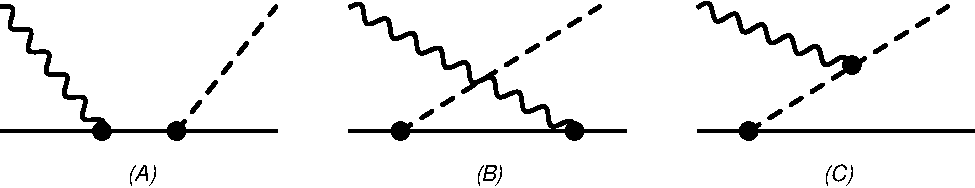
\epsfig{file=NucleonCrossSections.pdf,height=2.5cm,angle=0} 
\caption{Diagrams of the leading $\ga^\ast N \to  \pi N$ channel. \label{Fig:DiagsOp}}
\end{center}
\end{figure*}

\begin{figure}[tbh]
    \centering 
  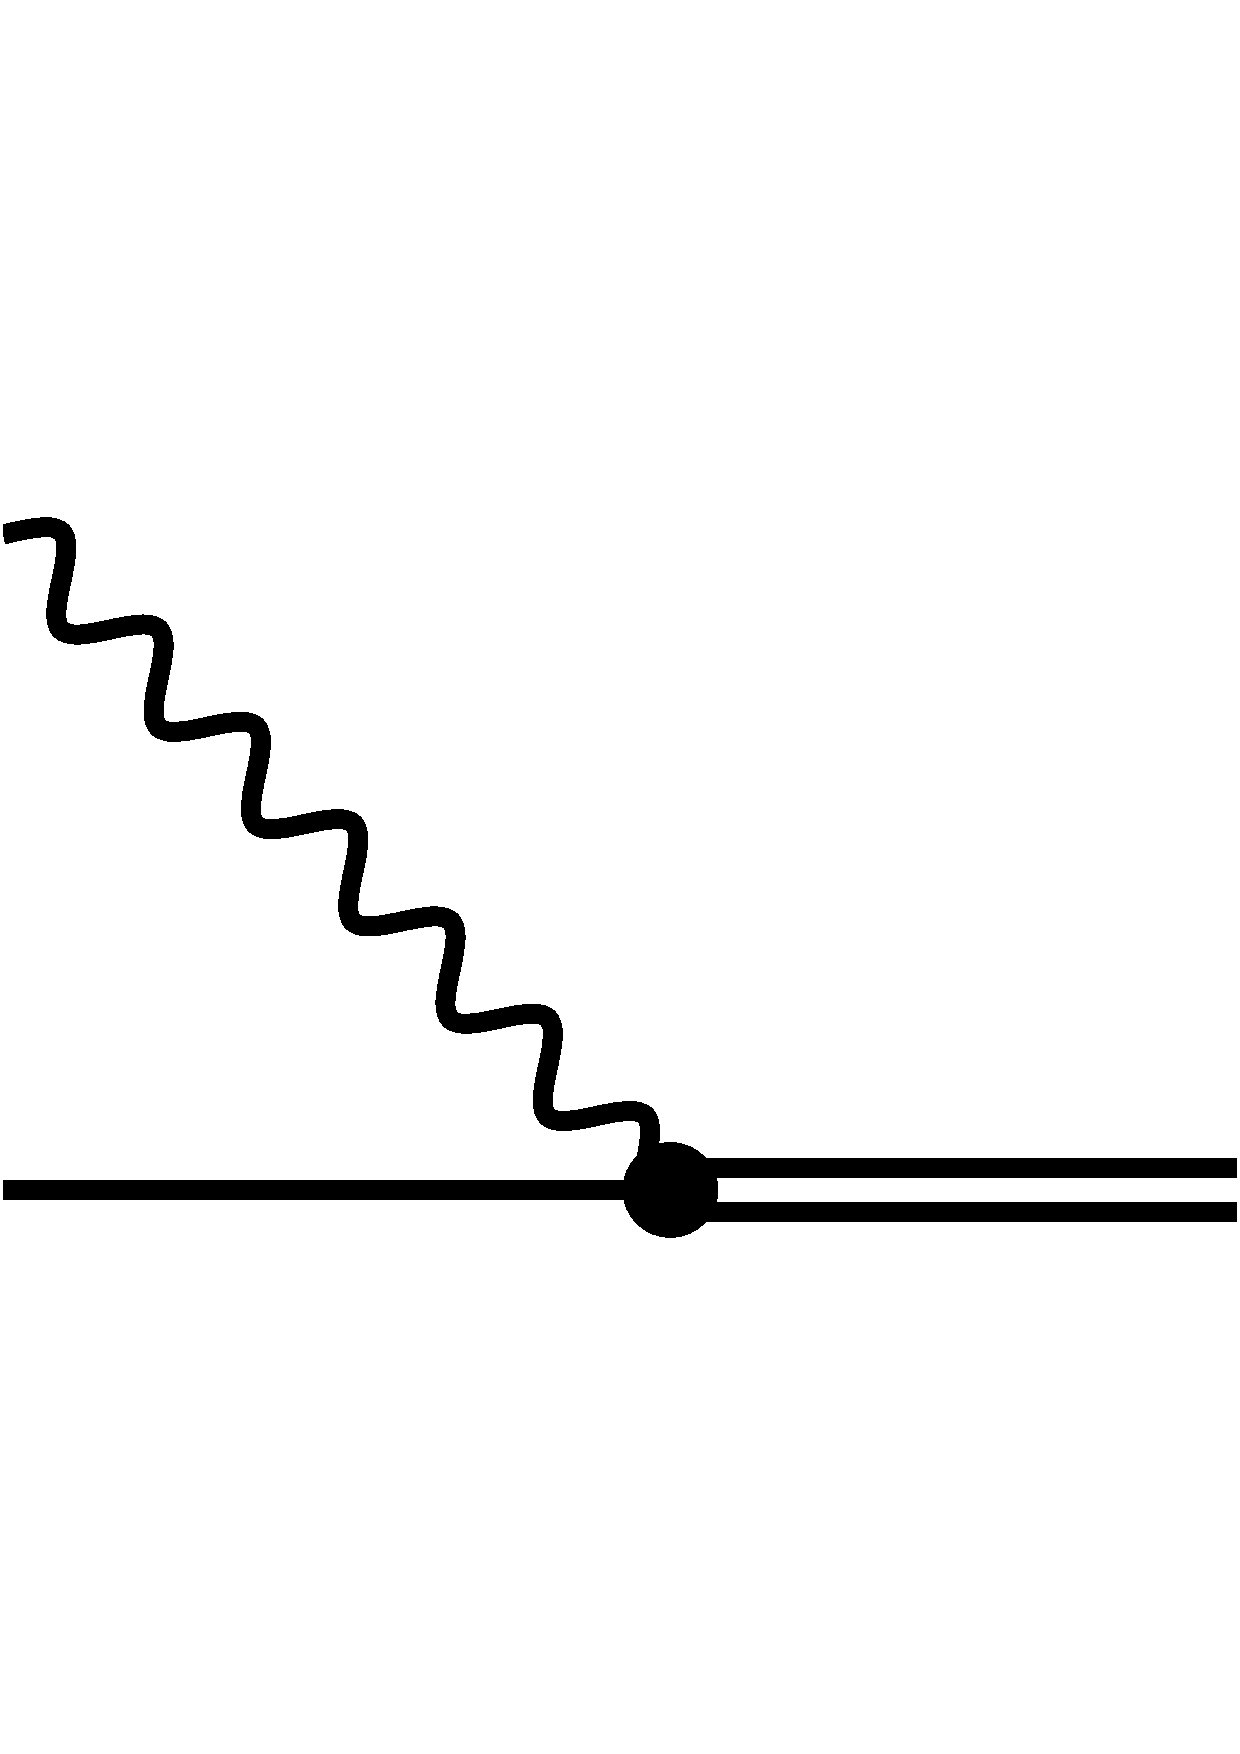
\includegraphics[height=2cm]{DeltaExchangeCrossSection.pdf}
\caption{The $\Delta(1232)$ production channel.\label{fig:CrossSectionDeltaProd}}
\end{figure}

\begin{figure*}[tbh]
\begin{center}
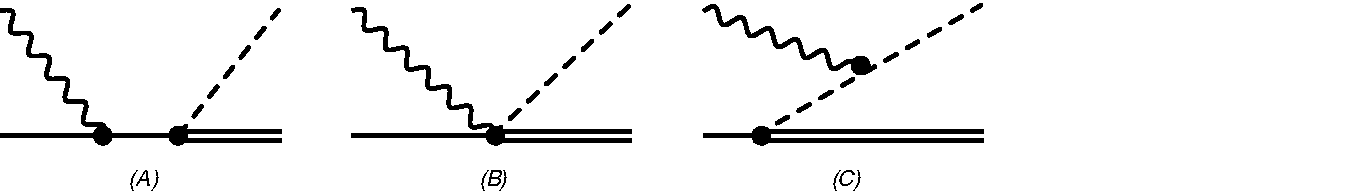
\epsfig{file=DeltaCrossSections.pdf,height=2.5cm,angle=0} 
\caption{Diagrams of the $\ga^\ast N\to \pi\Delta$ channel. \label{Fig:DiagsDeltaCS}}
\end{center}
\end{figure*}

At LO, we follow Refs.~\cite{Holstein:2005db,Lensky:2009uv} and perform a chiral rotation to cancel exactly the Kroll-Ruderman term at this order.
Therefore, we have to consider only the diagrams shown in Fig.~\ref{Fig:DiagsOp}, which are gauge invariant by themselves. We  checked that they reproduce the known results in the real-photon limit \cite{Lensky:2009uv,Holstein:2005db}.

The obtained cross sections were used to verify  the dispersion relations \Eqref{genDRs}  in B$\chi$PT. We checked that the non-Born VVCS amplitudes at LO, the left-hand side of \Eqref{genDRs}, are reproduced by the right-hand side of the same equation when the leading pion electroproduction cross sections are inserted. Analytical expressions for the latter can be found in Ref.~\cite{Alarcon:2013cba}. 

Besides the leading $\pi N$-production cross sections, we calculated the $\pi \Delta$-production cross sections, see Fig.~\ref{Fig:SummaryCrossSections}. Due to the worse high-energy behaviour of the $\pi \Delta$-production cross sections, the dispersion relations require further subtractions for a reconstruction of the $\pi \Delta$-loop contribution to VVCS.

The $\Delta$-production cross sections are related to the tree-level $\Delta$-exchange shown in Fig.~\ref{DeltaExchange}. The threshold for production of the $\Delta(1232)$-resonance is at lab-frame photon energies of:
\beq
\nu_\Delta=\frac{M_\Delta^2-M_N^2+Q^2}{2M_N}.
\eeq
Therefore, the $\Delta$-production cross sections contain to the following Dirac's $\de$-function: $\delta(\nu-\nu_\Delta)$. The
explicit form of these cross sections is given by:
\bea
\si_T(\nu,Q^2)&=&\frac{4\pi^2 \al}{2M_NM_+^2\vert \vec{q}\,\vert}\Bigg\{g_M^2 \vert \vec{q}\, \vert ^2 (\nu +M_+)+\frac{g_E^2\, (\nu -\varDelta ) \left(M_N\nu -Q^2\right)^2}{M_N^2}\\
&&+\frac{g_C^2 \,Q^4 s (\nu -\varDelta )}{M_N^2 M_\Delta^2}-\frac{g_M g_E\, \vert \vec{q}\, \vert ^2 \left(M_N\nu -Q^2\right)}{M_N}+\frac{g_M g_C\, \vert \vec{q}\, \vert ^2 Q^2}{M_N}\nn\\
&&+\frac{2 g_E g_C \,Q^2 \left(M_N\nu -Q^2\right) [-M_\Delta(M_N+\nu)+s]}{M_N^2 M_\Delta}\Bigg\}\delta\!\left(\nu-\nu_\Delta\right),\nn\\
\si_L(\nu,Q^2)&=&\frac{4\pi^2 \al}{2M_N^3M_+^2\vert \vec{q}\,\vert}\Bigg\{g_E^2(\nu-\varDelta)\left[M_N^2 \vert \vec{q}\, \vert^2-(Q^2-M_N\nu)^2\right]\\
&&+\frac{g_C^2 Q^2(\nu-\varDelta)(M_N^2 \vert \vec{q}\, \vert^2-Q^2 s)}{M_\Delta^2}\nn\\
&&-\frac{2 g_E g_C \,Q^2 \left(M_N\nu -Q^2\right) [s-M_\Delta(M_N+\nu)]}{ M_\Delta}\Bigg\}\delta\!\left(\nu-\nu_\Delta\right),\nn
\eea
with $\varDelta=M_\Delta - M$, $M_+=M_\Delta + M$ and the Mandelstam variable $s=M_N^2+2M_N \nu-Q^2$.
Analytical expressions for the unpolarized structure functions can be constructed with the help of \Eqref{VVCSunitarity}, with the flux factor $K(\nu,Q^2)=\sqrt{\nu^2+Q^2}$.

It is important to note that the above cross sections only describe the $\Delta$-pole contributions to the tree-level $\Delta$ exchange. In general, the VVCS amplitudes described by the $\Delta$-exchange diagram in Fig.~\ref{DeltaExchange} can be split as follows \cite{Hagelstein:2018bdi}:
\bea
\ol T_1^{\Delta\text{-exch.}}(\nu,Q^2)&=&\ol T_1^{\Delta\text{-exch.}}(0,Q^2)+T_1^{\Delta\text{-pole}}(\nu,Q^2)+\widetilde T_1^{\Delta\text{-exch.}}(\nu,Q^2),\qquad\;\\
\ol T_2^{\Delta\text{-exch.}}(\nu,Q^2)&=&T_2^{\Delta\text{-pole}}(\nu,Q^2)+\widetilde T_2^{\Delta\text{-exch.}}(\nu,Q^2).
\eea
$\ol T_1^{\Delta\text{-exch.}}(0,Q^2)$ is the usual subtraction function:
\bea
\ol T_1^{\Delta\text{-exch.}}(0,Q^2)&=&\frac{4\pi \al Q^4}{M_\Delta M_+ \omega_+}\left[\frac{g_M^2}{Q^2}-\frac{g_E^2 \varDelta}{M_N^2 M_+}-\frac{g_C^2 \varDelta \left(M_N^2-Q^2\right)}{M_N^2 M_\Delta^2 M_+}+\frac{g_M g_E}{M_N M_+}+\frac{g_M g_C}{M_N M_+}\right.\eqlab{T1su}\\
&&+\left.\frac{2 g_E g_C \left(M_N\varDelta +Q^2\right)}{M_N^2 M_\Delta M_+}\right].\nn
\eea
with  $\omega_\pm=(M_\Delta^2-M^2\pm Q^2)/2M_\Delta$. $T_i^{\Delta\text{-pole}}$ are the $\Delta$-pole contributions which feature a pole at the $\Delta(1232)$-production threshold, and thus, are proportional to
\beq
\frac{1}{[s-M_\Delta^2][u-M_\Delta^2]}=\frac{1}{4M_N^2}\frac{1}{\nu_\Delta^2-\nu^2}, \eqlab{poleStruc}
\eeq
 where $s$ and $u$ are the usual Mandelstam variables. $\widetilde T_i^{\Delta\text{-exch.}}$ are the ($\Delta$-)non-pole terms in which the pole has cancelled out \cite{Hagelstein:2018bdi}:
 \bea
\widetilde T_1^{\Delta\text{-exch.}}(\nu,Q^2)&=&-\frac{4\pi \al  \nu^2}{M_N M_+^2}\left(g_M^2+g_E^2-g_M g_E\right),\eqlab{T1nonpole}\\
\widetilde T_2^{\Delta\text{-exch.}}(\nu,Q^2)&=&-\frac{4\pi \al Q^2}{M_N M_+^2}\left(g_M^2+g_E^2-g_M g_E+\frac{g_C^2 Q^2}{M_\Delta^2}\right).\eqlab{T2nonpole}
\eea
 The non-pole terms in Eqs.~(\ref{eq:T1nonpole}) and (\ref{eq:T2nonpole}) can be described within the standard dispersive framework, \Eqref{genDRs}, with the structure functions:
\bea
\widetilde F_1(x,Q^2)&=&\frac{M_N x}{8 \pi \al} \,\widetilde T_1^{\Delta\text{-exch.}}(x,Q^2)\, \delta (x),\\
\widetilde F_2(x,Q^2)&=&\frac{Q^2}{16 \pi \al M_N} \,\widetilde T_2^{\Delta\text{-exch.}}(x,Q^2)\, \delta (x).
\eea

\begin{figure*}[tbh]
\begin{center} 
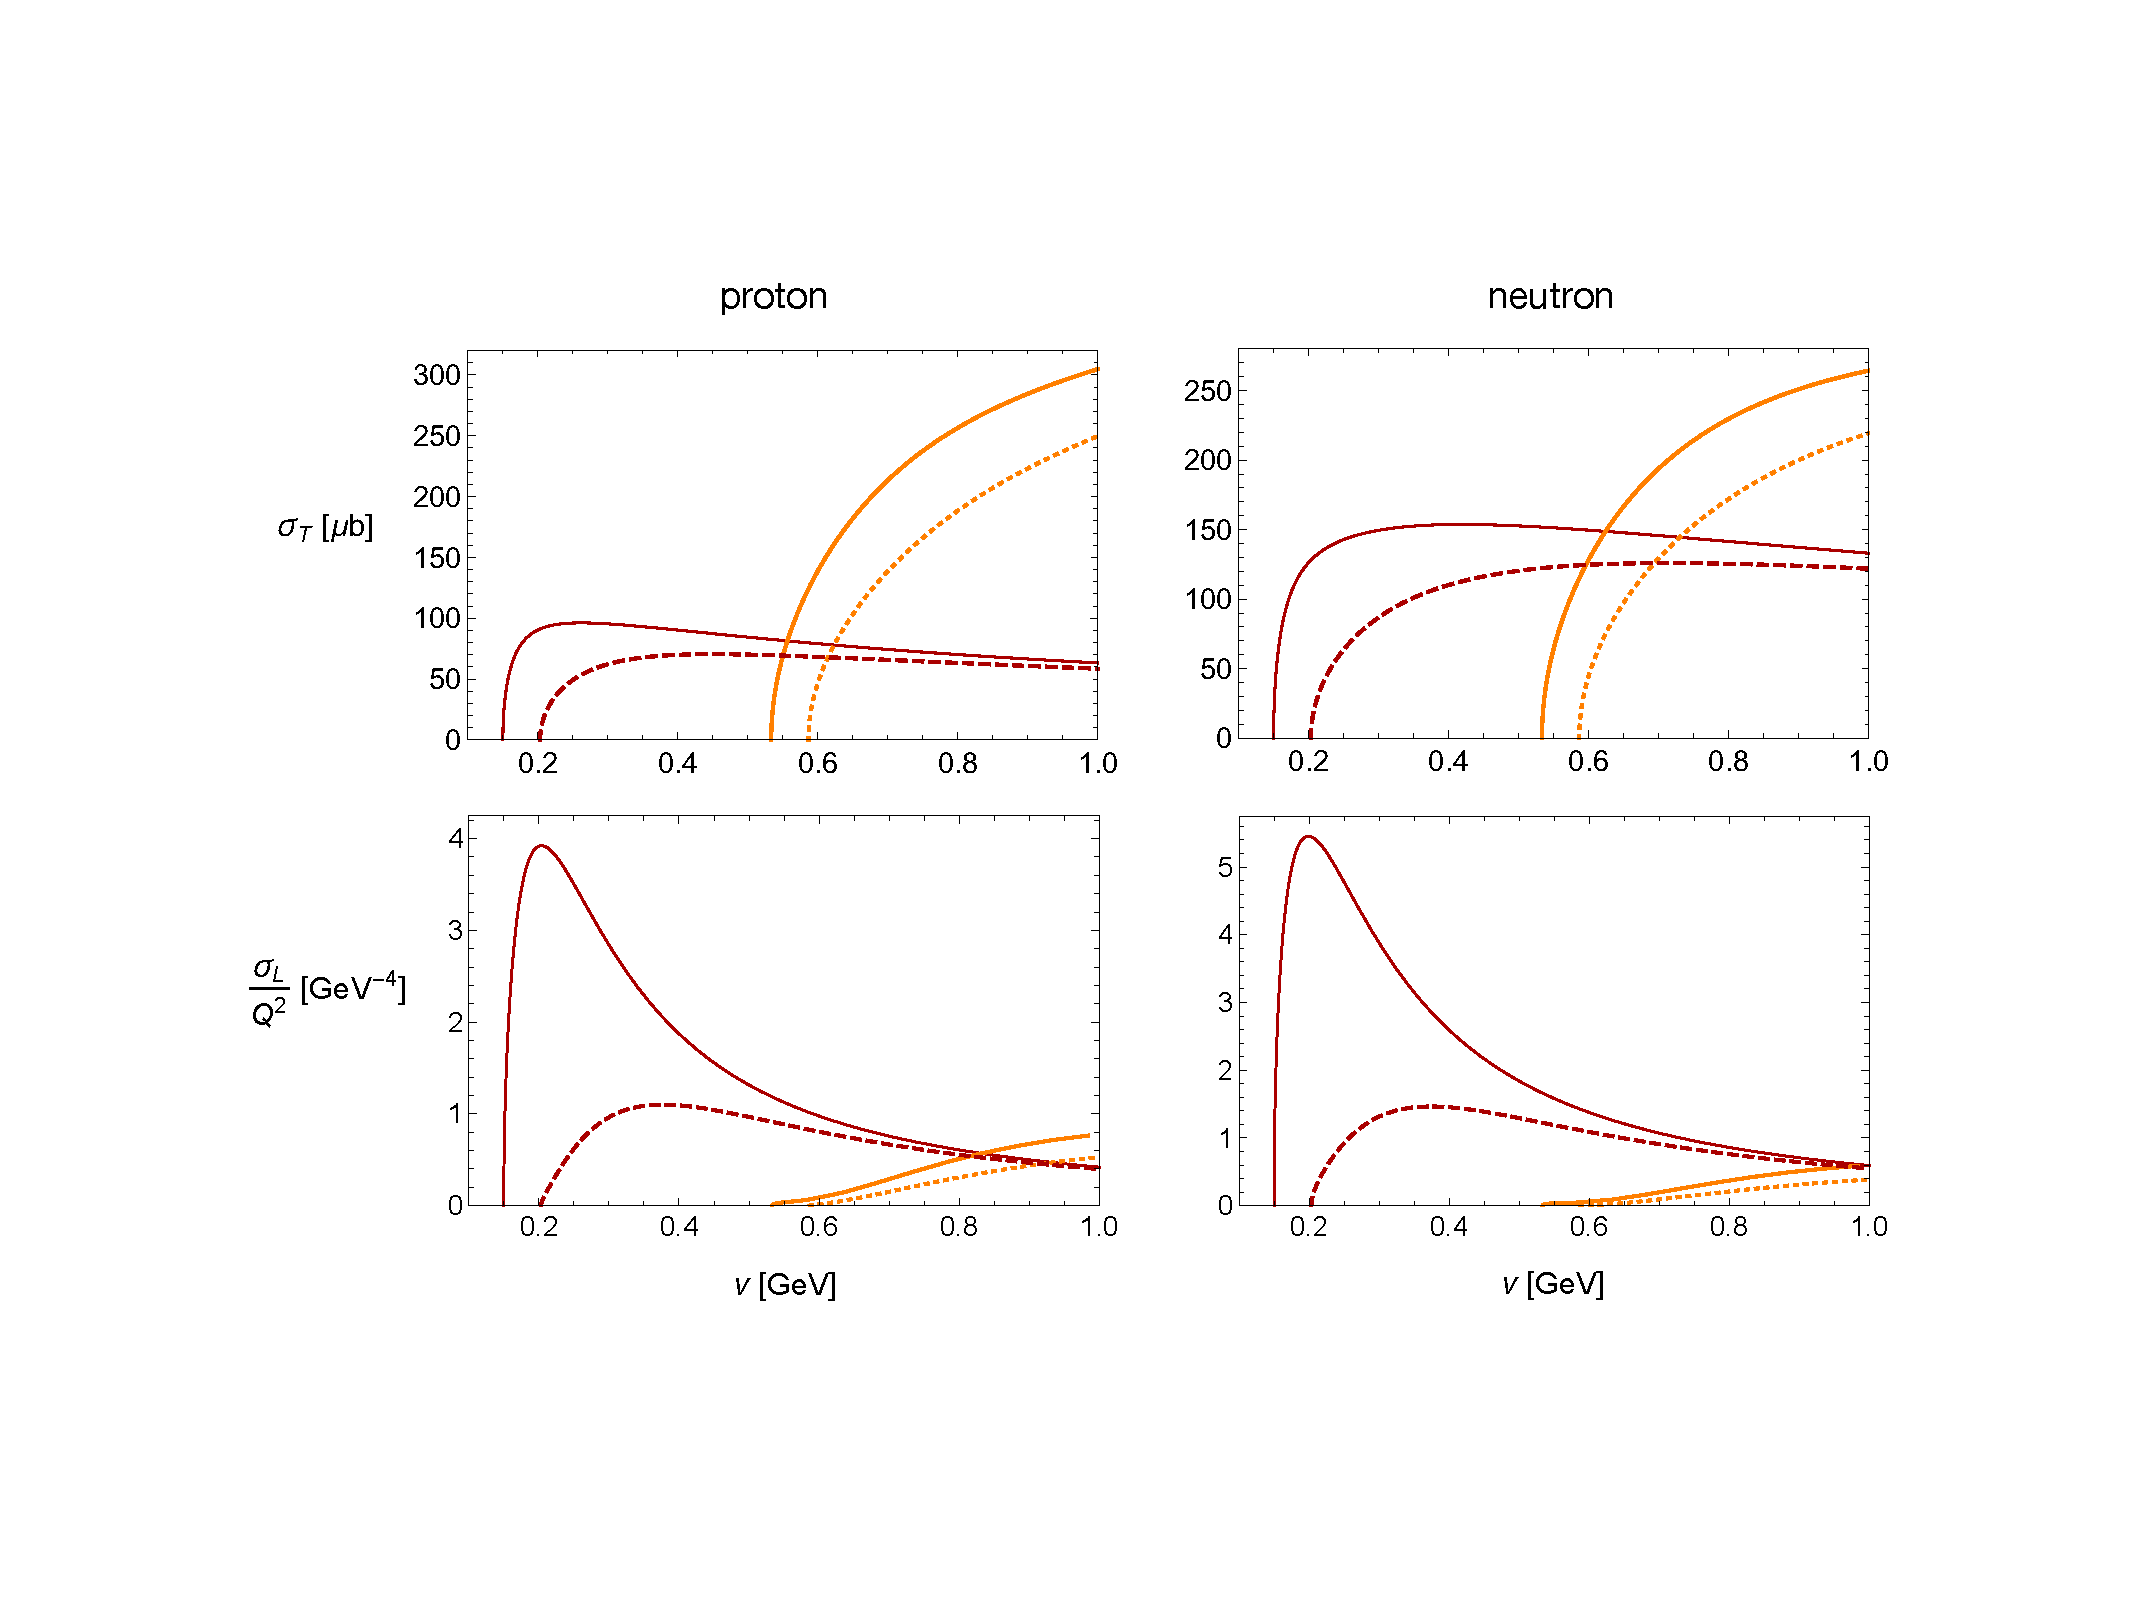
\includegraphics[width=0.95\textwidth]{UnpolarizedCrossSections.pdf}
\caption{Photoabsorption cross sections for $\pi N$ (red) and $\pi \Delta$ production (orange) with $Q^2=0$ (solid) and $Q^2=0.1$ GeV$^2$ (dashed for $\pi N$ and dotted for $\pi \Delta$ channel). \label{Fig:SummaryCrossSections}}
\end{center}
\end{figure*}

\section{Laboratory-frame decomposition of the VVCS amplitude}
\seclab{SRVVCStensor}
In the laboratory frame, the forward VVCS amplitude can be parametrized,
in terms of the nucleon Pauli matrices $\vec{\sigma}$, by four scalar functions $f_L$, $f_T$,
$g_{TT}$, and $g_{LT}$:
%\bea\label{Eq:T-Compt-definition}
%T(\nu,Q^2)&=&\eta\eta'\,f_{L}(\nu,Q^2) +(\vec{\epsilon}^{\,\, \prime *} \cdot \vec{\epsilon}\,) \,f_{T}(\nu,Q^2)  +  i \vec{\sigma}\cdot (\vec{\epsilon}^{\,\, \prime *} \times \vec{\epsilon}\,)\, g_{TT}(\nu,Q^2) \\
%&&-  i \vec{\sigma}\cdot [(\eta\,\vec{\epsilon}^{\,\, \prime *} - \vec{\epsilon}\,\eta')\times \hat{q}]\, g_{LT}(\nu,Q^2)\,.\nn 
%\eea
%This decomposition distinguishes between the longitudinal and transverse photons. Here, $\vec\epsilon$ ($\vec\epsilon^{\,\,\prime}$) is the incoming (outgoing) transverse photon polarization three-vector, $q$ is the photon four-momentum, $Q^2=-q^2$ is the virtuality of the photon and $\nu=(s-M_N^2+Q^2)/2M_N$ is the energy of the photon in the lab system.
%The coefficients $\eta$ and $\eta'$ correspond to the initial or final photon,
%respectively, and are equal to one (zero) if the photon is longitudinal (transverse).
\bea\label{Eq:T-Compt-definition}
T(\nu,Q^2)&=&\varepsilon_0\varepsilon_0^{\,\prime*}\,f_{L}(\nu,Q^2) +(\vec{\varepsilon}^{\,\, \prime *} \cdot \vec{\varepsilon}\,) \,f_{T}(\nu,Q^2)  +  i \vec{\sigma}\cdot (\vec{\varepsilon}^{\,\, \prime *} \times \vec{\varepsilon}\,)\, g_{TT}(\nu,Q^2) \\
&&-  i \vec{\sigma}\cdot [(\varepsilon_0\vec{\varepsilon}^{\,\, \prime *} - \vec{\varepsilon}\,\varepsilon^{\,\prime *}_0)\times \hat{q}]\, g_{LT}(\nu,Q^2)\,.\nn 
\eea
Here, $Q^2=-q^2$ is the virtuality of the photon with $q$ being the photon four-momentum, $\nu=(s-M_N^2+Q^2)/2M_N$ is the energy of the photon in the lab system, $\vec q$ and $\hat{q}=\vec{q}/\vert \vec{q}\, \vert$ are the photon three-momentum in the lab system and its unit vector. The modified polarization vector components are given by
\begin{align}
\varepsilon_0&=\left[\epsilon_0-\frac{\nu}{\left|\vec q\,\right|}\, (\vec\epsilon\cdot\hat q\,)\right]\frac{\left|\vec q\,\right|}{Q}\,,
&\vec\varepsilon = \vec\epsilon-\hat q\,(\vec\epsilon\cdot\hat q\,)\,,\eqlab{modified_polarization_vectors}
\end{align}
 where $\epsilon=(\epsilon_0,\vec\epsilon\,)$ is the polarization vector of the initial photon; the primed vector corresponds to the final photon.

The amplitudes, $f_T$ and $f_L$, are independent of the nucleon spin and are
related to the amplitude of the  manifestly-covariant form of \eqref{Eq:T-Rel} as:
\begin{subequations}
\begin{align}
  f_T(\nu,Q^2) &= T_1(\nu,Q^2), \label{Eq:fT-T1}\\
  f_L(\nu,Q^2) &= - T_1(\nu,Q^2) +  \frac{\nu^2 + Q^2}{Q^2} T_2(\nu,Q^2), \label{Eq:fL-T1T2}
  %\\
 %g_{TT}(\nu, Q^2) &= \frac{\nu}{M_N}\Big[ S_1(\nu,Q^2) - \frac{Q^2}{M_N\,\nu} S_2(\nu,Q^2)\Big],\label{Eq:gTT-S1S2}\\
%  g_{LT}(\nu, Q^2) &= \frac{Q}{M_N}\Big[ S_1(\nu,Q^2) + \frac{\nu}{M_N} S_2(\nu,Q^2)\Big].\label{Eq:gLT-S1S2}
\end{align} 
\end{subequations}





The polarizabilities can then be obtained from linear combinations of the non-Born contributions  $\ol T_1$ and $\ol T_2$. 
\bea
\left(\ol T_1(\nu,\,Q^2)-\ol T_1(0,\,Q^2)\right)/4\pi 
&=&
M^{(2)}_{1}(Q^2)  \, \nu^2 \,+\, M^{(4)}_{1}(Q^2)  \, \nu^4 \,+\,{\mathcal{O}}(\nu^6) \,,
\label{eq:T1lex}\\
\ol T_2(0,Q^2)/4\pi =  Q^2 M_2^{(1)}(Q^2) ,
\label{eq:T20}
\eea
where
\beq 
M_i^{(n)}  = 
\eeq 
Note that $\al_{E1}+\be_{M1} = M^{(2)}_{1}(0)=M^{(1)}_{2}(0)$, and 
$\alpha_L = M^{(1)\prime}_2(0)  - M^{(2)\prime}_1(0) 
+ M^{(4)}_1(0)$.




\section{Polarizabilities at $Q^2=0$}\label{App:PolarizabilitiesAll}


\subsection{$\pi N$-loop  contribution}
\label{App:Polarizabilities}

Here we give the analytical expressions for the $\pi N$-loop contributions to the proton and neutron polarizabilities, expanded
in powers of $\mu = m_\pi/M_N$, viz., the HB expansion. We
choose to expand here to a high order in $\mu$, the strict
HB expansion would only retain the leading term in an analogous
NLO calculation. The complete expressions can be found in the {\it Supplemented material}.


\bea
\alpha_{E1}^{(p)}+\beta_{M1}^{(p)} &=& 
%\frac{e^2 g_A^2}{96\pi^3 f_\pi^2\,  (4-\mu^2)^{5/2} m_\pi} \left\{ \mu \sqrt{4-\mu^2} \left[  2 (\mu^2-4)^2(18 \mu^4 -35\mu^2 + 9) \log\mu -36 \mu^6 + 304 \mu^4 \right.\right. \nonumber \\
%& \left.\left. - 737 \mu^2+ 406 \right] + 2 \left[-18\mu^{10}+ 215 \mu^8 - 899 \mu^6 + 1500 \mu^4 - 788\mu^2 + 44\right] \arctan\left( \frac{\sqrt{4-\mu^2}}{\mu} \right)\right\} \nonumber \\
  \frac{e^2 g_A^2}{96\pi^3 f_\pi^2\, m_\pi} \left\{  \frac{11 \pi }{8} + 6  (3 \log \mu +4)\mu - \frac{1521 \pi \mu^2}{64} -\frac{ (210 \log \mu + 29)\mu^3 }{3  } \right. \\ 
&&\left.+ \frac{ 32625 \pi \mu^4 }{1024 }+ \frac{ 9 (80 \log \mu - 67)\mu^5 }{20  }+\dots\right\},\nn\\
\alpha_{E1}^{(n)}+\beta_{M1}^{(n)} &=& 
%\frac{e^2 g_A^2}{48\pi^3 f_\pi^2\,  (4-\mu^2)^{5/2} m_\pi} \left\{ 3 \mu \sqrt{4-\mu^2} \left[  (\mu^2-4)^2 \log\mu+5-\mu^2 \right]\right. \nonumber \\
%& \left. + \left[44-86\mu^2+30\mu^4 -3 \mu^6 \right] \arctan\left( \frac{\sqrt{4-\mu^2}}{\mu} \right)\right\} \nonumber \\
 \frac{e^2 g_A^2}{96\pi^3 f_\pi^2\, m_\pi} \left\{  \frac{11 \pi}{8} + \frac{ (12 \log \mu +1)\mu}{2} - \frac{117 \pi \mu^2}{64} +\frac{ 7 \mu^3 }{3 } - \frac{ 375\pi \mu^4 }{1024 }\right. \\
 &&\left.+ \frac{ 3 \mu^5 }{5 }+\dots\right\},\nn
\eea




\bea
\alpha_{L}^{(p)} &=&
%\frac{e^2 g_A^2}{1440 \pi^3 f_\pi^2\,  (4-\mu^2)^{9/2} m_\pi^3}\left\{   \mu  \sqrt{4-\mu^2} [ 6 \mu^2 (4-\mu^2)^4 (85 - 178 \mu^2 + 78 \mu^4) \log\mu -10648  \nonumber \right.\\
%&+ 141550 \mu^2- 241775 \mu^4 + 161138 \mu^6 -51252 \mu^8 + 7854 \mu^{10} -468 \mu^{12}  ]  - 6 [-496 - 11596  \mu^2  \nonumber \\
%&\left.+ 91796 \mu^4 -167484 \mu^6 + 134610 \mu^8 - 56718 \mu^{10} + 13117 \mu^{12} - 1582 \mu^{14} + 78 \mu^{16}] \arctan\left( \frac{\sqrt{4-\mu^2}}{\mu}\right) \right\}\nonumber\\
 \frac{e^2 g_A^2}{1440 \pi^3 f_\pi^2\,  m_\pi^3}\left\{ \frac{93 \pi}{32} - \frac{89 \mu}{2} + \frac{18231 \pi \mu^2}{256} +10 (44+ 51 \log\mu )\mu^3 -\frac{1880805 \pi \mu^4}{4096} \right. \\
&&\left. - 3\left(356 \log\mu -\frac{129}{10}\right)\mu^5 +\dots  \right\},\nn\\
\alpha_{L}^{(n)} &= &
%\frac{e^2 g_A^2}{1440 \pi^3 f_\pi^2\,  (4-\mu^2)^{9/2} m_\pi^3}\Big\{   \mu  \sqrt{4-\mu^2} [ 60 \mu^2 (4-\mu^2)^4  \log\mu -3736 + 9270 \mu^2 - 4547 \mu^4  \nonumber\\
%& + 882 \mu^6 -60 \mu^8   ]  - 12 [-248 - 1086  \mu^2 + 3082 \mu^4 - 2090 \mu^6 + 630 \mu^8 - 90 \mu^{10} + 5 \mu^{12}] \nonumber \\
%&\times\arctan\left( \frac{\sqrt{4-\mu^2}}{\mu}\right) \Big\}\nonumber \\
 \frac{e^2 g_A^2}{1440 \pi^3 f_\pi^2\,  m_\pi^3}\left\{ \frac{93 \pi}{32} - \frac{35}{2} \mu + \frac{4095 \pi \mu^2}{256} + \frac{1}{2}(11+ 120 \log\mu )\mu^3 -\frac{80085 \pi \mu^4}{4096}\right. \\
 &&\left.+ \frac{141\mu^5}{5} +\dots  \right\},\nn
\eea


\bea
M_1^{(4)(p)} &=&\frac{e^2 g_A^2}{720 \pi^3 f_\pi^2 m_\pi^3}\left\{\frac{81 \pi}{32}-56 \mu+\frac{29145\pi\mu^2}{256}+\frac{3}{4}\left(1501+1380 \log \mu \right)\mu^3-\frac{4670925\pi \mu^4}{4096}\right.\\
&&\left.-\frac{96}{5}\left(13+160\log \mu\right)\mu^5\right\},\nn\\
M_1^{(4)(n)} &= &\frac{e^2 g_A^2}{720 \pi^3 f_\pi^2 m_\pi^3}\left\{\frac{81\pi}{32}-28\mu+\frac{6525\pi\mu^2}{256}+3\left(1+30\log \mu\right)\mu^3-\frac{113925\pi\mu^4}{4096}+\frac{192\mu^5}{5}\right\}
\eea






\bea
\left.\frac{\dd\left(\alpha_{E1}^{(p)}+\beta_{M1}^{(p)}\right) (Q^2)}{\dd Q^2}\right|_{Q^2=0}
%-\frac{e^2 g_A^2}{480 \pi^3 f_\pi^2\,  (4-\mu^2)^{7/2} m_\pi^3}\left\{ \mu\sqrt{4-\mu^2} [2\mu^2 (\mu^2-4)^3 (275-945 \mu^2  \right. \nonumber \\
%&+486 \mu^4) \log\mu + 1140-46942 \mu^2 + 91370 \mu^4-52795 \mu^6 +12096 \mu^8 -972 \mu^{10} ]  -2 [24 +6456\mu^2 \nonumber\\
%&\left. -91068 \mu^4 +185570 \mu^6 - 138040 \mu^8 +47525\mu^{10} -7749\mu^{12} +486 \mu^{14}] \arctan\left( \frac{\sqrt{4-\mu^2}}{\mu}\right) \right\} \nonumber \\
&=& \frac{e^2 g_A^2}{480 \pi^3 f_\pi^2\,  m_\pi^3} \left\{  \frac{3 \pi}{16} -18 \mu + \frac{6477 \pi \mu^2}{128} + \left( \frac{1339}{2} + 550 \log\mu\right)\!\mu^3 \right.  \\ 
&& \left. -\frac{1366515 \pi \mu^4}{2048}-7\left( \frac{313}{10} + 270 \log\mu  \right)\mu^5 +\dots  \right\},\nonumber\\
\left.\frac{\dd\left(\alpha_{E1}^{(n)}+\beta_{M1}^{(n)}\right) (Q^2)}{\dd Q^2}\right|_{Q^2=0}&=&
%\frac{e^2 g_A^2}{1440 \pi^3 f_\pi^2\,  (4-\mu^2)^{4} m_\pi^3}\left\{ \mu(\mu^2-4) [150\mu^2 (\mu^2-4)^3  \log\mu \right. \nonumber \\
%& +2812-4942 \mu^2 + 1551 \mu^4-150 \mu^6]  + 6 \sqrt{4-\mu^2}[24+1824 \mu^2 - 3530 \mu^4 + 1750 \mu^6 \nonumber \\
%&\left.-350 \mu^8 + 25 \mu^{10}] \arctan\left( \frac{\sqrt{4-\mu^2}}{\mu}\right) \right\} \nonumber \\
 \frac{e^2 g_A^2}{1440 \pi^3 f_\pi^2\,  m_\pi^3} \left\{  \frac{9 \pi}{16} -\frac{89 \mu}{2} + \frac{5535 \pi \mu^2}{128} + \left( 1+ 150 \log\mu\right)\mu^3 \right.\\
 &&\left.-\frac{92265  \pi \mu^4}{2048}  +  \frac{1209 \mu^5}{20} +\dots  \right\}\nn
\eea




\bea
\left.\frac{\dd\alpha_{L}^{(p)} (Q^2)}{\dd Q^2}\right|_{Q^2=0}&=& \frac{e^2 g_A^2}{1440 \pi^3 f_\pi^2  m_\pi^5}\left\{-\frac{621\pi}{896}+\frac{13\mu}{14}+\frac{4995\pi \mu^2}{1024} - \frac{669\mu^3}{7}\right.\\
&&\left.+\frac{2517315\pi\mu^4}{16384}+ ( \frac{34407}{35} + 1116 \log \mu)\mu^5\right\}\nn\\
%\frac{e^2 g_A^2}{720 \pi f_\pi^2 (4-\mu^2)^{9/2} m_\pi^3}\left\{\mu  \sqrt{4-\mu ^2} \left(-468 \mu ^{12}+7854 \mu ^{10}-51252 \mu ^8 + 161138 \mu ^6  \right. \right. \nonumber\\
%&\left. - 241775 \mu ^4 +141550 \mu ^2+6 \left(\mu ^2-4\right)^4  \left(78 \mu ^4-178 \mu ^2+85\right) \mu ^2 \log (\mu )-10648\right)-6 \left(78 \mu ^{16}-1582 \mu ^{14}  \right. \nonumber \\
 %& \left. \left.+13117 \mu ^{12}-56718 \mu   ^{10} +134610 \mu ^8-167484 \mu ^6+91796 \mu ^4-11596 \mu ^2-496\right) \cot ^{-1}\left(\frac{\mu }{\sqrt{4-\mu ^2}}\right)\right\}
\left.\frac{\dd\alpha_{L}^{(n)} (Q^2)}{\dd Q^2}\right|_{Q^2=0}&=&\frac{e^2 g_A^2}{1440 \pi^3 f_\pi^2  m_\pi^5}\left\{-\frac{621\pi}{896}-\frac{55\mu}{14}+\frac{3195\pi\mu^2}{1024}-\frac{207\mu^3}{7}+\frac{456915\pi\mu^4}{16384}\right.\\
&&\left.+\frac{18}{35}(29+210 \log \mu)\mu^5\right\}\nn
%\frac{e^2 g_A^2}{10080 \pi ^3 f_\pi^2 m_\pi^5 (4-\mu ^2)^6} (12 \sqrt{4-\mu ^2} (\mu ^2 ((7 (9 \mu ^2 (\mu ^8-22 \mu ^6+198 \mu ^4-924 \mu^2 \nonumber \\ 
%&  +2310)-24928) \mu ^2 +55102) \mu ^2+9732)-1656) \cot ^{-1}(\frac{\mu }{\sqrt{4-\mu^2}})+\mu  (\mu ^2-4) (-756 \mu ^{12}  \nonumber \\
%&  + 13968 \mu ^{10}-100464 \mu ^8+343893 \mu ^6 -524272 \mu ^4+148400 \mu ^2+756 (\mu ^2-4)^5 \mu ^4 \log (\mu )+33128))
\eea

\bea
\left.\frac{\dd M_2^{(1)(p)} }{\dd Q^2}\right|_{Q^2=0}&=&\frac{e^2 g_A^2}{480\pi^3 f_\pi^2 m_\pi^3}\left\{-\frac{17\pi}{32}+\frac{9\mu}{2}-\frac{399\pi\mu^2}{256}+\frac{1}{3}\left(197+90\log \mu\right)\mu^3-\frac{246015\pi\mu^4}{4096}\right.\\
&&\left.-\frac{1}{5}\left(199+990\log \mu\right)\mu^5\right\},\nn\\
\left.\frac{\dd M_2^{(1)(n)} }{\dd Q^2}\right|_{Q^2=0}&=&\frac{e^2 g_A^2}{480\pi^3 f_\pi^2 m_\pi^3}\left\{-\frac{17\pi}{32}-2\mu+\frac{705\pi\mu^2}{256}+\frac{1}{6}\left(1+60\log \mu\right)\mu^3-\frac{12255\pi\mu^4}{4096}\right.\\
&&\left.+\frac{79\mu^5}{20}\right\}\nn
\eea

\bea
\left.\frac{\dd M_1^{(4)(p)} }{\dd Q^2}\right|_{Q^2=0}&=&\frac{e^2g_A^2}{10080\pi^3f_\pi^2m_\pi^5}\left\{\frac{225\pi}{128}-229\mu+\frac{495555\pi\mu^2}{1024}-7542\mu^3+\frac{217523775\pi\mu^4}{16384}\right.\\&&+3\left(38771+37408\log \mu\right)\mu^5\Bigg\},\nn\\
\left.\frac{\dd M_1^{(4)(n)} }{\dd Q^2}\right|_{Q^2=0}&=&\frac{e^2g_A^2}{2520\pi^3f_\pi^2m_\pi^5}\left\{\frac{225\pi}{512}-\frac{209\mu}{4}+\frac{228795\pi\mu^2}{4096}-\frac{1653\mu^3}{4}+\frac{21341775\pi\mu^4}{65536}\right.\\
&&+3\left(3+364\log \mu\right)\mu^5\Bigg\}\nn
\eea

\subsection{ $\Delta$-exchange contribution}\seclab{DeltaTreePolarizabilities}



In this section, we give analytical expressions for the  tree-level $\Delta$-exchange contributions, cf.\ Fig.~\ref{DeltaExchange}, to the nucleon polarizabilities and their slopes at $Q^2=0$. Note that the $\Delta$-exchange  contributes equally to proton and neutron polarizabilities. The $\gamma^* N \Delta$ vertex follows from the Lagrangian given in \Eqref{gammaNDeltaLag}:
\bea
%\Gamma_{\Delta \rightarrow \gamma N}^{\al \mu}&=&-\sqrt{\frac{3}{2}}\frac{e}{M(M+M_\Delta)}\left\{g_M \gamma^{\al \mu \kappa \lambda}p'_\kappa q_\lambda+g_E(p'\cdot q\, g^{\al \mu}-q^\al p^{\prime\mu})\right.\\
%&&\left.-\frac{g_C}{M_\Delta} \left(q^2 g^{ \al \mu}\slashed{p}'-q^2 p^{\prime\mu} \gamma^\al +p'\cdot q \,q^\mu \gamma^\al-q^\al q^\mu \slashed{p}'\right)\right\}\gamma_5,\qquad\nn\\
\Gamma_{\gamma N \rightarrow \Delta}^{\al \mu}&=&\sqrt{\frac{3}{2}}\frac{e}{M_N M_+}T_3^\dagger\left\{g_M \gamma^{\al \mu \kappa \lambda}p'_\kappa q_\lambda+g_E (p'\cdot q\, g^{\al \mu}-q^\al p^{\prime\mu})\right.\\
&&\left.+\frac{g_C}{M_\Delta} \left(q^2 g^{ \al \mu}\slashed{p}'-q^2 p^{\prime\mu} \gamma^\al +p'\cdot q \,q^\mu \gamma^\al-q^\al q^\mu \slashed{p}'\right)\right\}\gamma_5,\qquad\nn
\eea
with $p+q=p'$, where $p$, $q$ and $p'$ are the momenta of nucleon, photon and Delta, respectively. In what follows we use $\varDelta = M_\Delta - M_N$, $M_+=M_\Delta+M_N$. The masses and coupling constants are given in Table \ref{tab:constants}.  Recall that for the magnetic $\gamma N \Delta $ coupling, we introduced the vector-meson-dominance dependence: $g_M \rightarrow g_M/(1+Q^2/\Lambda^2)^2$. The analytical expressions for $\Delta$-exchange contribution are given below.


\bea
\eqlab{alphabetaQ2}
\al_{E1}&=&-\frac{e^2 g_E^2}{2 \pi  M_+^3}\\
\be_{M1}&=&\frac{e^2 g_M^2}{2 \pi  \varDelta  M_+^2}
\eea

\beq
\al_L=\frac{e^2 M_\Delta^2}{\pi M_+^3}\left(\frac{ g_E^2}{\varDelta  M_NM_+^2}-\frac{g_C^2}{2 M_\Delta^4}+\frac{ g_E g_C}{M_NM_\Delta^2 M_+}\right)
\eeq

\bea
M_1^{(4)}&=&\frac{e^2 M_N}{\pi M_+^3 \varDelta} \left(\frac{g_M^2}{\varDelta^2}+\frac{g_E^2}{M_+^2}-\frac{g_E g_M}{\varDelta M_+}\right)
\eea

\bea
\frac{\dd \left[\alpha_{E1}(Q^2)+\beta_{M1}(Q^2)\right]}{\dd Q^2}\Bigg\vert_{Q^2=0}&=&-\frac{e^2}{\pi M_+^2}\left(\frac{g_M^2}{\varDelta^2}\left[\frac{1}{M_+}-\frac{1}{2\varDelta}\right]+\frac{2}{ \Lambda^2 }\frac{g_M^2}{\varDelta}\right.+\frac{g_M g_E}{M_N}\left[\frac{1}{4\varDelta^2}\right.\\
&&\left.-\frac{1}{\varDelta M_+}+\frac{1}{4M_+^2}\right] -\frac{g_E^2}{4M_NM_+}\left[\frac{1}{\varDelta}-\frac{5}{M_+}\right]\nn\\
&&\left.-\frac{ g_M g_C}{2  \varDelta  M_NM_+}+\frac{g_E g_C}{M_NM_+^2}\right)\nn
\eea

\bea
\frac{\dd \al_L(Q^2)}{\dd Q^2}\Bigg\vert_{Q^2=0}&=&\frac{e^2 M_\Delta^3}{\pi \varDelta M_+^4}\left(\frac{2g_E^2}{\varDelta^2 M_+^2}\left[\frac{2}{M_\Delta}-\frac{1}{M_N}\right]-\frac{g_C^2}{ M_\Delta^4}\left[\frac{1}{M_N}-\frac{3}{2M_\Delta}\right]\right.  \\
&&+\left.\frac{g_E g_C}{\varDelta M_\Delta^2 M_+}\left[\frac{5}{M_\Delta}-\frac{3}{M_N}\right]\right)\nn
\eea

\bea
\left.\frac{\dd M_2^{(1)} }{\dd Q^2}\right|_{Q^2=0}&=&\frac{e^2 }{\pi M_+^3}\left(-\frac{g_M^2}{2\varDelta^2}-\frac{2g_M^2 M_+}{\Lambda^2 \varDelta}+\frac{g_M g_E}{2\varDelta M_N }+\frac{g_E^2}{2\varDelta M_+}+\frac{g_M g_C}{2\varDelta M_N}-\frac{g_C^2}{2M_\Delta^2}\right)
\eea

\bea
\left.\frac{\dd M_1^{(4)} }{\dd Q^2}\right|_{Q^2=0}&=&\frac{e^2 M_N}{\pi \varDelta^2 M_+^5}\left(\frac{g_M^2}{\varDelta}\left[2-\frac{5M_+}{\varDelta}+\frac{M_+^2}{\varDelta^2}\right]-\frac{4M_+^2}{\varDelta}\frac{g_M^2}{\Lambda^2}+g_M g_E \left[\frac{6}{\varDelta}-\frac{M_+}{\varDelta^2}-\frac{1}{M_+}\right]\right.\\
&&\left.+\frac{2M_+ g_M g_E}{\Lambda^2}+g_E^2\left[\frac{1}{\varDelta}-\frac{7}{M_+}\right]+\frac{2g_M g_C}{\varDelta}-\frac{4g_E g_C}{M_+}\right)\nn
\eea


\newpage

%\begin{spacing}{0.8}
  \small
\bibliography{lowQ}
%\end{spacing}



\end{document}